\documentclass[10pt]{beamer}

\usetheme[progressbar=frametitle]{metropolis}
\usepackage{appendixnumberbeamer}
\metroset{sectionpage=none}

\usepackage{multirow}
\usepackage{caption}
\usepackage{subcaption}

\usepackage{tzplot}
\usepackage{booktabs}
\usepackage[scale=2]{ccicons}

\usepackage{pgfplots}
\usepgfplotslibrary{dateplot,fillbetween}

\usepackage{xspace}
\newcommand{\themename}{\textbf{\textsc{metropolis}}\xspace}

\usepackage{tikz} 
\usetikzlibrary{arrows,shapes,tikzmark,decorations.pathreplacing,calc,fit,positioning,matrix,chains}

\usepackage{hyperref}
\usepackage{multimedia}

\usepackage{graphicx} % Load graphics
\usepackage{booktabs} % Nice tables
\usepackage{dcolumn} % Booktabs column spacing
\usepackage{threeparttable} % Align column caption, table, and notes
\usepackage{adjustbox} % Shrink stuff
\usepackage{makecell}
%\usepackage{showframe} % Useful for debugging



% *****************************************************************
% Estout LaTeX wrapper
% *****************************************************************

%%Original code developed by Jörg Weber: see
%% https://www.jwe.cc/2012/03/stata-latex-tables-estout/
%% and
%% https://www.jwe.cc/blog/


\let\estinput=\input % define a new input command so that we can still flatten the document

\newcommand{\estwide}[3]{
		\vspace{.75ex}{
			%\textsymbols% Note the added command here
			\begin{tabular*}
			{\textwidth}{@{\hskip\tabcolsep\extracolsep\fill}l*{#2}{#3}}
			\toprule
			\estinput{#1}
			\\ \bottomrule          % 08 Dec 2021. Add these slashes.
			\addlinespace[.75ex]
			\end{tabular*}
			}
		}	

\newcommand{\estauto}[3]{
		\vspace{.75ex}{
			%\textsymbols% Note the added command here
			\begin{tabular}{l*{#2}{#3}}
			\toprule
			\estinput{#1}
			\\ \bottomrule          % 08 Dec 2021. Add these slashes.
			\addlinespace[.75ex]
			\end{tabular}
			}
		}

% Allow line breaks with \\ in specialcells
\newcommand{\specialcell}[2][c]{%
    \begin{tabular}[#1]{@{}c@{}}#2\end{tabular}
}

\newcommand{\sym}[1]{\rlap{#1}}% Thanks David Carlisle


%%%%%%%%%%% End of wrapper %%%%%%%%%%%%%%%%%%%%%



\title{Learning about in-group or out-group facts and the role of the presenter.}
%\subtitle{A modern beamer theme}
% \date{\today}
\date{August 14, 2023}
\author{Luisa Carrer}
\institute{University of Zurich}
% \titlegraphic{\hfill\includegraphics[height=1.5cm]{logo.pdf}}

\begin{document}

\maketitle

\section[Introduction]{Introduction}

\begin{frame}{Introduction}
\begin{columns}
    \column{0.35\textwidth}
    \begin{tikzpicture}[scale = 0.5]
 \only<1-2>{
\node[inner sep=0pt] (info) at (0,-4)
    {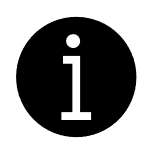
\includegraphics[width=.25\textwidth]{info_black.png}};
\node[inner sep=0pt] (person) at (3.5,0)
    {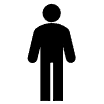
\includegraphics[width=.25\textwidth]{person_black.png}};
\node[inner sep=0pt] (presenter) at (7,-4)
    {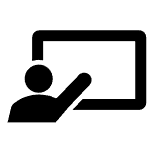
\includegraphics[width=.25\textwidth]{presenter_black.png}};
   } 
 \only<2>{   
\draw[<->,thick] (person.south west) -- (info.north east);
\draw[<->,thick] (info.east) -- (presenter.west);
\draw[<->,thick] (person.south east) -- (presenter.north west);
}
\end{tikzpicture}
 \only<3>{   
\begin{figure}[h!]
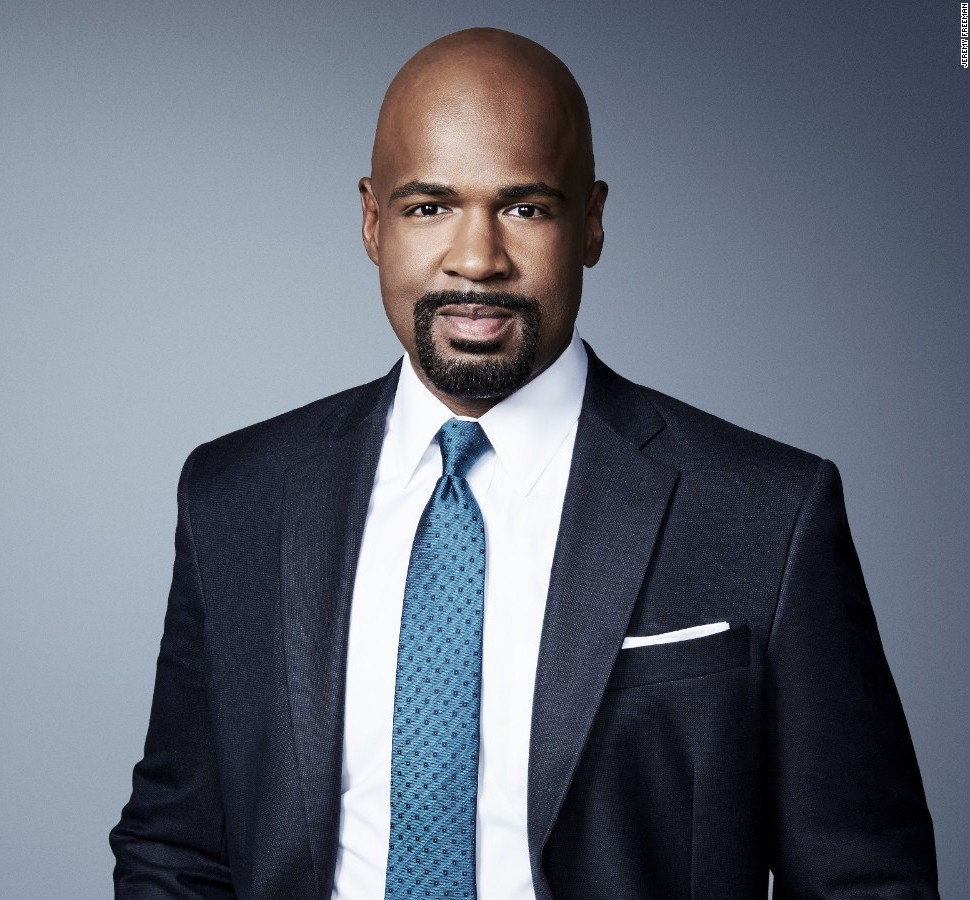
\includegraphics[width=3.5cm]{img/pic/Blackwell originaljpg.jpg} \\
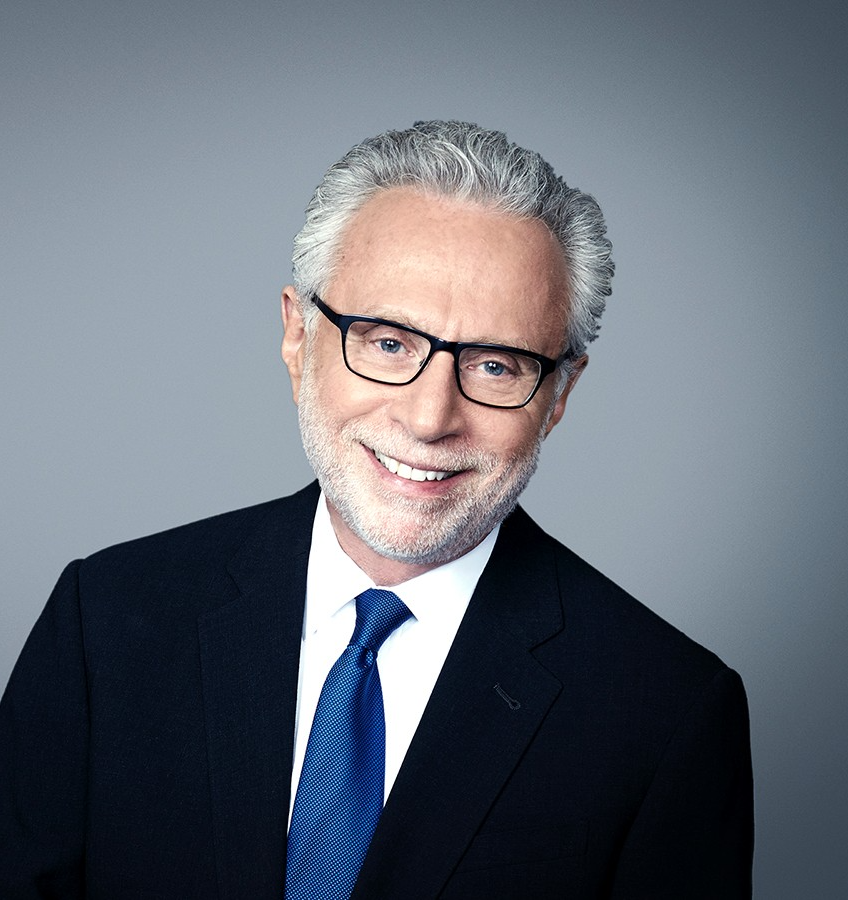
\includegraphics[width=3.5cm]{img/pic/wolf-blitzer-cropped.png}
\end{figure}
}
    \column{0.65\textwidth}
\begin{itemize}
 \only<1->{  \item Most communication have at least three components} \only<1>{:
            \begin{enumerate}
                \item Presenter
                \item Receiver
                \item Information Content
            \end{enumerate}}
 \only<2->{   \item What happens when these three components share identity?     }  

\only<3->{\item E.g., what happens if Blackwell vs. Blitzer were to present BLM?} 
\end{itemize}
    \end{columns}
\end{frame}





\begin{frame}{Research Questions}
\label{RQ}

\begin{columns}
    \column{0.25\textwidth}{
\begin{tikzpicture}[scale = 0.4]
\node[inner sep=0pt] (info) at (0,-4)
    {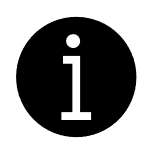
\includegraphics[width=.25\textwidth]{info_black.png}};
\node[inner sep=0pt] (person) at (3.5,0)
    {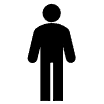
\includegraphics[width=.25\textwidth]{person_black.png}};
\node[inner sep=0pt] (presenter) at (7,-4)
    {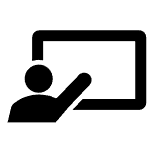
\includegraphics[width=.25\textwidth]{presenter_black.png}};
\draw[<->,thick] (person.south west) -- (info.north east);
\draw[<->,thick] (info.east) -- (presenter.west);
\draw[<->,thick] (person.south east) -- (presenter.north west);    
\end{tikzpicture}
}
\column{0.7\textwidth}{
How are misperception and learning rates affected when
\begin{itemize}
\item[Q1] there is congruence between presenter and audience?
\item[Q2] there is congruence between audience and information content?
\item[Q3] there is congruence between presenter and information content?
    
\end{itemize}
}
\end{columns}
\end{frame}


\begin{frame}{Overview}
  \setbeamertemplate{section in toc}[sections numbered]
    \begin{block}{Structure}
  \tableofcontents[hideallsubsections]
  \end{block}
  \vskip
  \begin{block}{Preview of findings}
      \item No effect when audience = presenter
      \item Positive effect on learning (negative on misperceptions) when audience = info
      \item Positive effect on learning (negative on misperceptions) when presenter = info
  \end{block}
\end{frame}



\begin{frame}{Literature}
\label{Lit}
\begin{block}{Misperceptions about others}
\begin{itemize}
    \item For a review, Bursztyn and Yang (forthcoming)
  \item[->] \textit{Study a mechanism for misperceptions and potential solution} 
\end{itemize}
\end{block}
\begin{block}{Concordance between Audience and Presenter}
    \begin{itemize}
    \item Previous studies find conflicting results on the effect of concordance between audience and presenter on persuasion  (e.g., Alsan and Eichmeyer, 2021; D’Acunto
et al., 2021)
    \item[->] \textit{Study how information subject matter interacts with presenter and audience}
    \end{itemize}
\end{block}
\begin{block}{Behavioral Inattention}
\begin{itemize}
   % \item  Consumers do not fully attend to prices when consuming different goods (e.g. Lacetera et al., 2012), limited attention to freely available financial news (e.g. DellaVigna and Pollet, 2007, 2009)
    \item[->] \textit{Inattention to out-group information, and whether it varies according to whom presents it}
\end{itemize}
\end{block}
\end{frame}






\section{Experimental Design}

\begin{frame}[fragile]{Design}
    \begin{itemize}
		\item Online information provision experiment
            \item Timeline:
            	
	    \begin{center}
    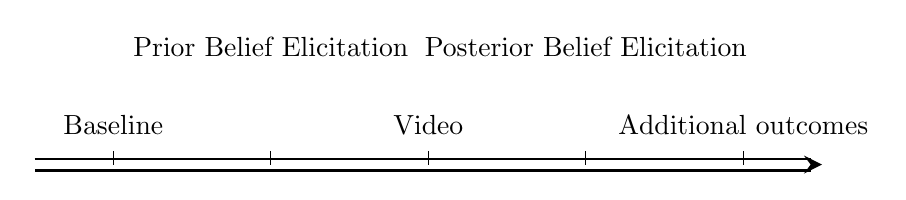
\begin{tikzpicture}
    
        % draw horizontal line   
    \draw[->, line width=1pt, double distance=3pt] (-5,0) -- (5,0);
    
    
    % draw vertical lines
    \foreach \x in {-4,-2,0,2,4}
    \draw (\x cm,5pt) -- (\x cm,0pt);
    
    % draw nodes
    \node at (-4,0.5) {Baseline};
     \node at (-2,1.5){Prior Belief Elicitation};
     \node at (2,1.5){Posterior Belief Elicitation};
     \node at (0,0.5){Video};
     \node at (4,0.5){Additional outcomes};

\end{tikzpicture}
\end{center} 

            \items Beliefs about 9 statistical health-related facts
                    \begin{itemize}
                    \item 4 facts about racial subpopulations (Black Americans, White Americans, Asian Americans, Hispanic Americans)
                    \item Posteriors beliefs: "what was \alert{mentioned} in the video?"
                    \end{itemize}

		\item Standard belief experiment
		\begin{itemize}
		    \item Priors and posteriors about signals are incentivezed via BSR  
		    \item Minimal description (as suggested by Danz et al. (2020))
		\end{itemize}
		\item Subjects are randomly assignes to watch a video
		
	\end{itemize}


\end{frame}


  
  \begin{frame}{Video}
\label{Video_info}

	\begin{columns}
	\column{0.55\textwidth}
		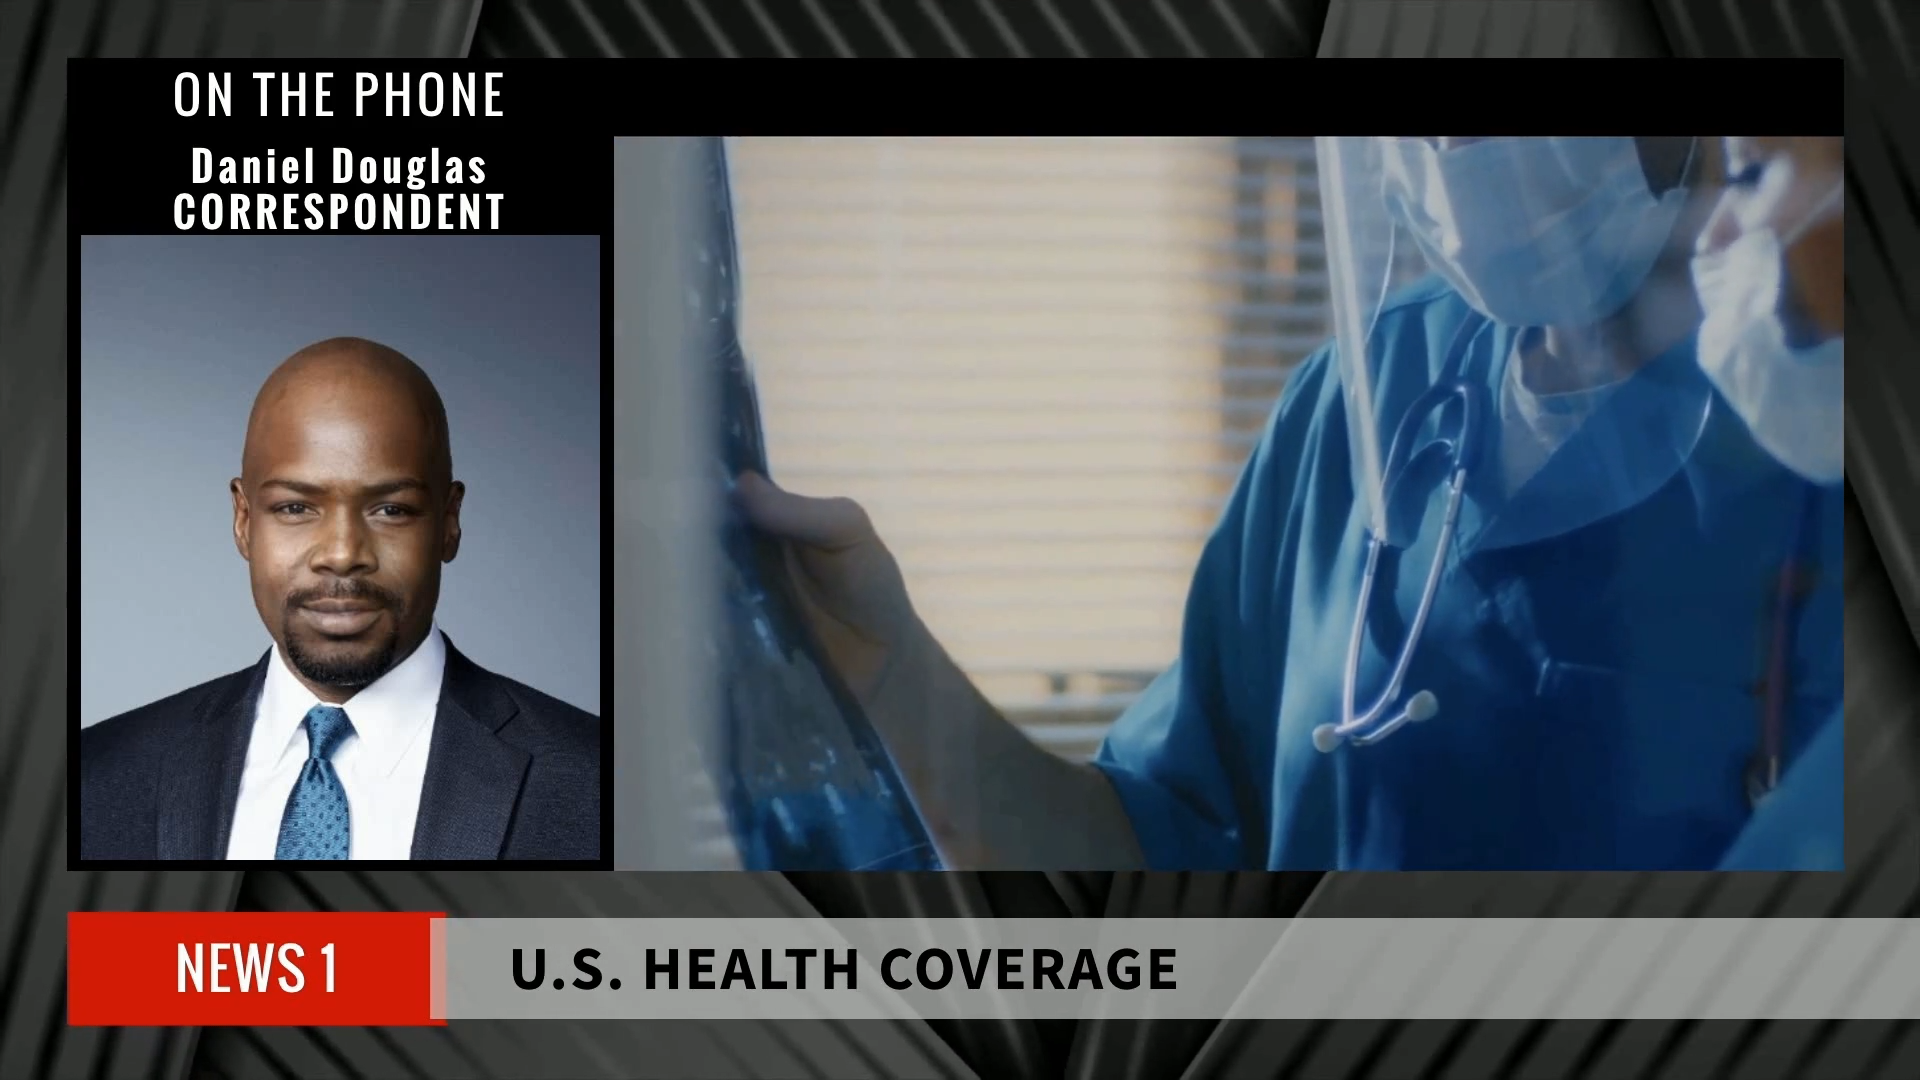
\includegraphics[width=1\textwidth]{img/Frame-13-08-2023-09-04-37.png}
	\column{0.55\textwidth}
	\begin{itemize}
 		\item Video that mimics news segment on U.S. health insurance coverage and other health related issues
            \item Length video reports all facts for which priors and posteriors are elicited (3 min 45 sec)
	    \item Neutral male voice narrating script $\rightarrow$ race signal validated via experiment
	    \item Pictures signaling presenter's race (rather than using names)
	\end{itemize}
	\end{columns}
	
  \hfill \hyperlink{facts}{\beamerbutton{Facts}} \hyperlink{voice}{\beamerbutton{Voice}} 
  \hyperlink{cheating}{\beamerbutton{Cheating Avoidance}}
  % \beamerbutton{\href{https://vimeo.com/698712834/06223d499a}{Partial Video}}\beamerbutton{\href{https://vimeo.com/683581176/44de64427c}{Full Video}}
	

\end{frame}

  
\begin{frame}{Pictures - Signaling Race}
\label{pic examples}
\begin{columns}
    \column{0.5\textwidth}
\begin{figure}[h!]
\begin{minipage}{1\columnwidth}
\subfloat{
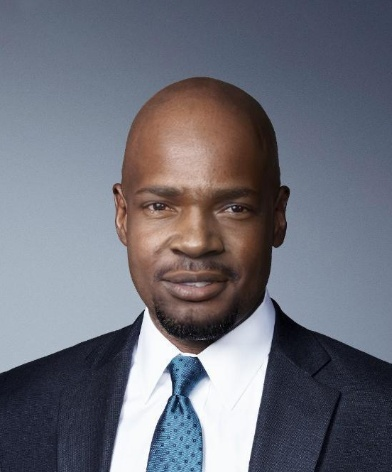
\includegraphics[height=3.5cm]{img/pic/blackwell-BM-017.jpg}
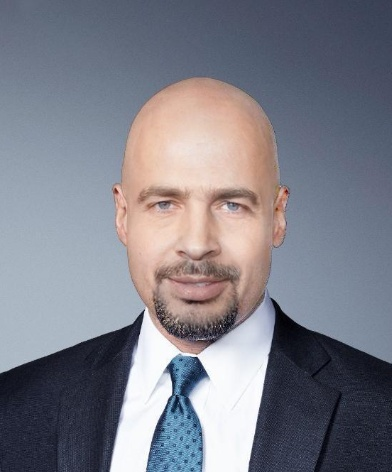
\includegraphics[height=3.5cm]{img/pic/blackwell-WM-018.jpg}}
\captionsetup[subfloat]{labelformat=empty}
\subfloat[Example of Resulting Pairs]{
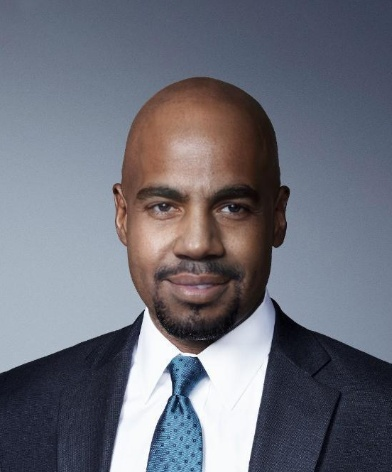
\includegraphics[height=3.5cm]{img/pic/blackwell-BM-208.jpg}
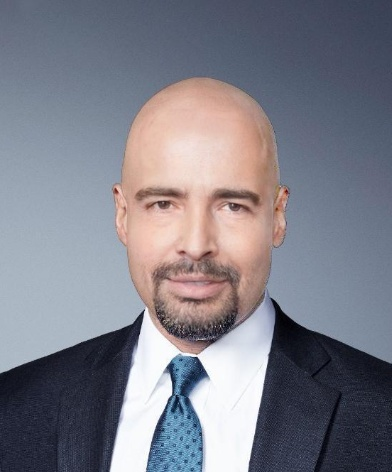
\includegraphics[height=3.5cm]{img/pic/blackwell-WM-211.jpg}}
\end{minipage}
\end{figure}

    \column{0.5\textwidth}
\begin{itemize}
\item Race signaled by picture \rightarrow avoid issues with signaling race with names
\item Created via AI-fact swapping tool and photo editing
\item Pair pictures in Face Chicago Dataset
\item Results in 42 pictures with varying race, but all other details kept extremely similar
\end{itemize}
\end{columns}
\vspace{-0.5cm}
\hfill \hyperlink{pic_Manipulation}{\beamerbutton{How}} \hyperlink{all_pic}{\beamerbutton{More}} 
\end{frame}




\section{Results}
\subsection{Data}
\begin{frame}{Sample}
\label{data}
\begin{itemize}
    \item Experiment run in July 2023, with 2062 individuals recruited via Prolific
    \item Limited to Black and White U.S. residents aged 18-65 who could undertake the survey on a computer
\end{itemize}
\hfill \hyperlink{balance}{\beamerbutton{Data}}
\end{frame}



\begin{frame}{Explanatory Variables: Congruence}

      \begin{description}
\item[congruence 1] congruence between \textbf{audience} and \textbf{presenter}. \\
    = 1 if Black respondent and Black presenter, or (White respondent and White presenter), 0 otherwise 
 \item[congruence 2] congruence between \textbf{audience} and \textbf{information} content. \\
    = 1 if Black respondent and Black population-related news, or (White respondent and White population-related news), 0 otherwise
 \item[congruence 3] congruence between \textbf{presenter} and \textbf{information} content. \\
    = 1 if Black presenter and Black population-related news, or (White presenter and White population-related news), 0 otherwise 
      \end{description}
\end{frame}


\begin{frame}{Outcomes}
\setbeamercovered{transparent}
\begin{block}{1. Misperceptions}<1>
Absolute difference between each reported posterior and the signal 
$\alert{M_{i,f}} = |po_{i,f} - s_f|$
\end{block}

\begin{block}{2. Learning Rate}<0>
Feedback from the signal onto the posterior.
\begin{equation*}
    po_{i,f} - pr_{i,f} = \alert{\beta} \left( s_f - pr_{i,f}\right)
    \label{eq: learningrate}
  \end{equation*}
\end{block}


\begin{description}
  \item[$po_{i,f}$] Respondent $i$'s elicited posterior about fact $f$
  \item[$pr_{i,f}$] Respondent $i$'s elicited prior about fact $f$
  \item[$s_f$] True value for fact $f$
\end{description}
\end{frame}




\subsection{Results}



\begin{frame}{Misperceptions}
\label{mainI}
\centering
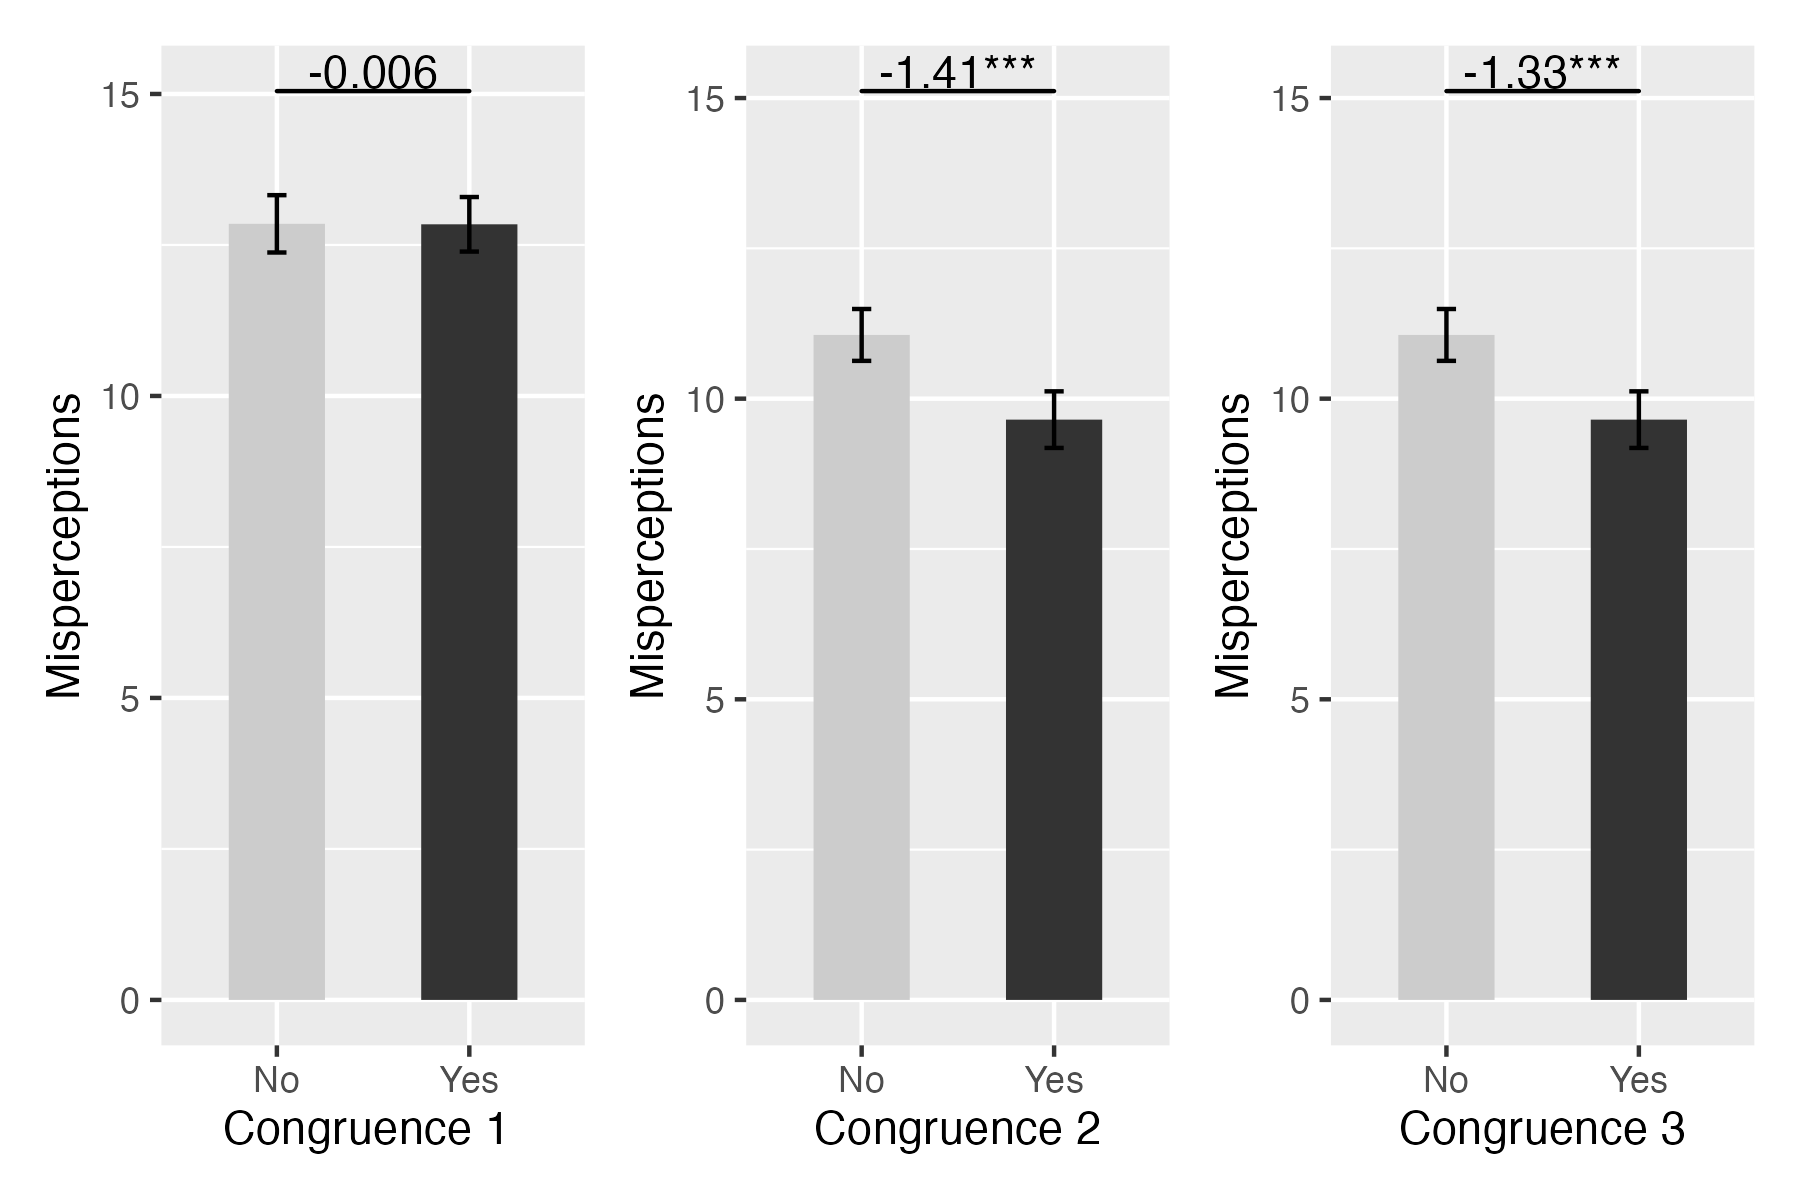
\includegraphics[height=6cm]{output/MainI.png}	
\begin{itemize}
\item No s.s. effect of congruence 1
\item Negative effect of congurence 2 and 3 on mispercepetions
\end{itemize}
\hfill \hyperlink{mainI_reg}{\beamerbutton{reg}}
\end{frame}

\begin{frame}{Outcomes}
\setbeamercovered{transparent}
\begin{block}{1. Misperceptions}<0>
Absolute difference between each reported posterior and the signal 
$\alert{M_{i,f}} = |po_{i,f} - s_f|$
\end{block}

\begin{block}{2. Learning Rate}<1>
Feedback from the signal onto the posterior.
\begin{equation*}
    po_{i,f} - pr_{i,f} = \alert{\beta} \left( s_f - pr_{i,f}\right)
    \label{eq: learningrate}
  \end{equation*}
\end{block}


\begin{description}
  \item[$po_{i,f}$] Respondent $i$'s elicited posterior about fact $f$
  \item[$pr_{i,f}$] Respondent $i$'s elicited prior about fact $f$
  \item[$s_f$] True value for fact $f$
\end{description}
\end{frame}


\begin{frame}{Learning Rate}
\label{eq_learning}
\begin{center}
\scalebox{0.8}{
\begin{tikzpicture}
\tzaxes(-0.5,-0.5)(3,3){$truth - prior$}{$posterior-prior$}
\tzfn[metropolis,thick]{\x}[-0.5:3]{$posterior = truth$}[ar]
\end{tikzpicture}
}
\end{center}
\begin{equation*}
    posterior_{i,f} - prior_{i,f} = \beta_0 \left( signal_{f} - prior_{i,f}\right)+  \beta_1 \left( signal_{f} - prior_{i,f}\right) *C^{j}
  \end{equation*}
      \begin{description}
\item[$posterior_{i,f}$]  elicited posterior about fact $f$ from individual $i$
\item[$prior_{i,f}$] elicited prior about fact $f$ from individual $i$
\item[$signal_{f}$] true value for fact $f$ reported in the video
\item[$C^{j}$] $\in [Congruence1, Congruence2, Congruence3]$ 
      \end{description}
\hfill \hyperlink{regressioneq}{\beamerbutton{Regression}}
\end{frame}




\begin{frame}{Learning Rates}
\label{mainII}
\begin{columns}
    \column{0.65\textwidth}
\only<1>{
\centering
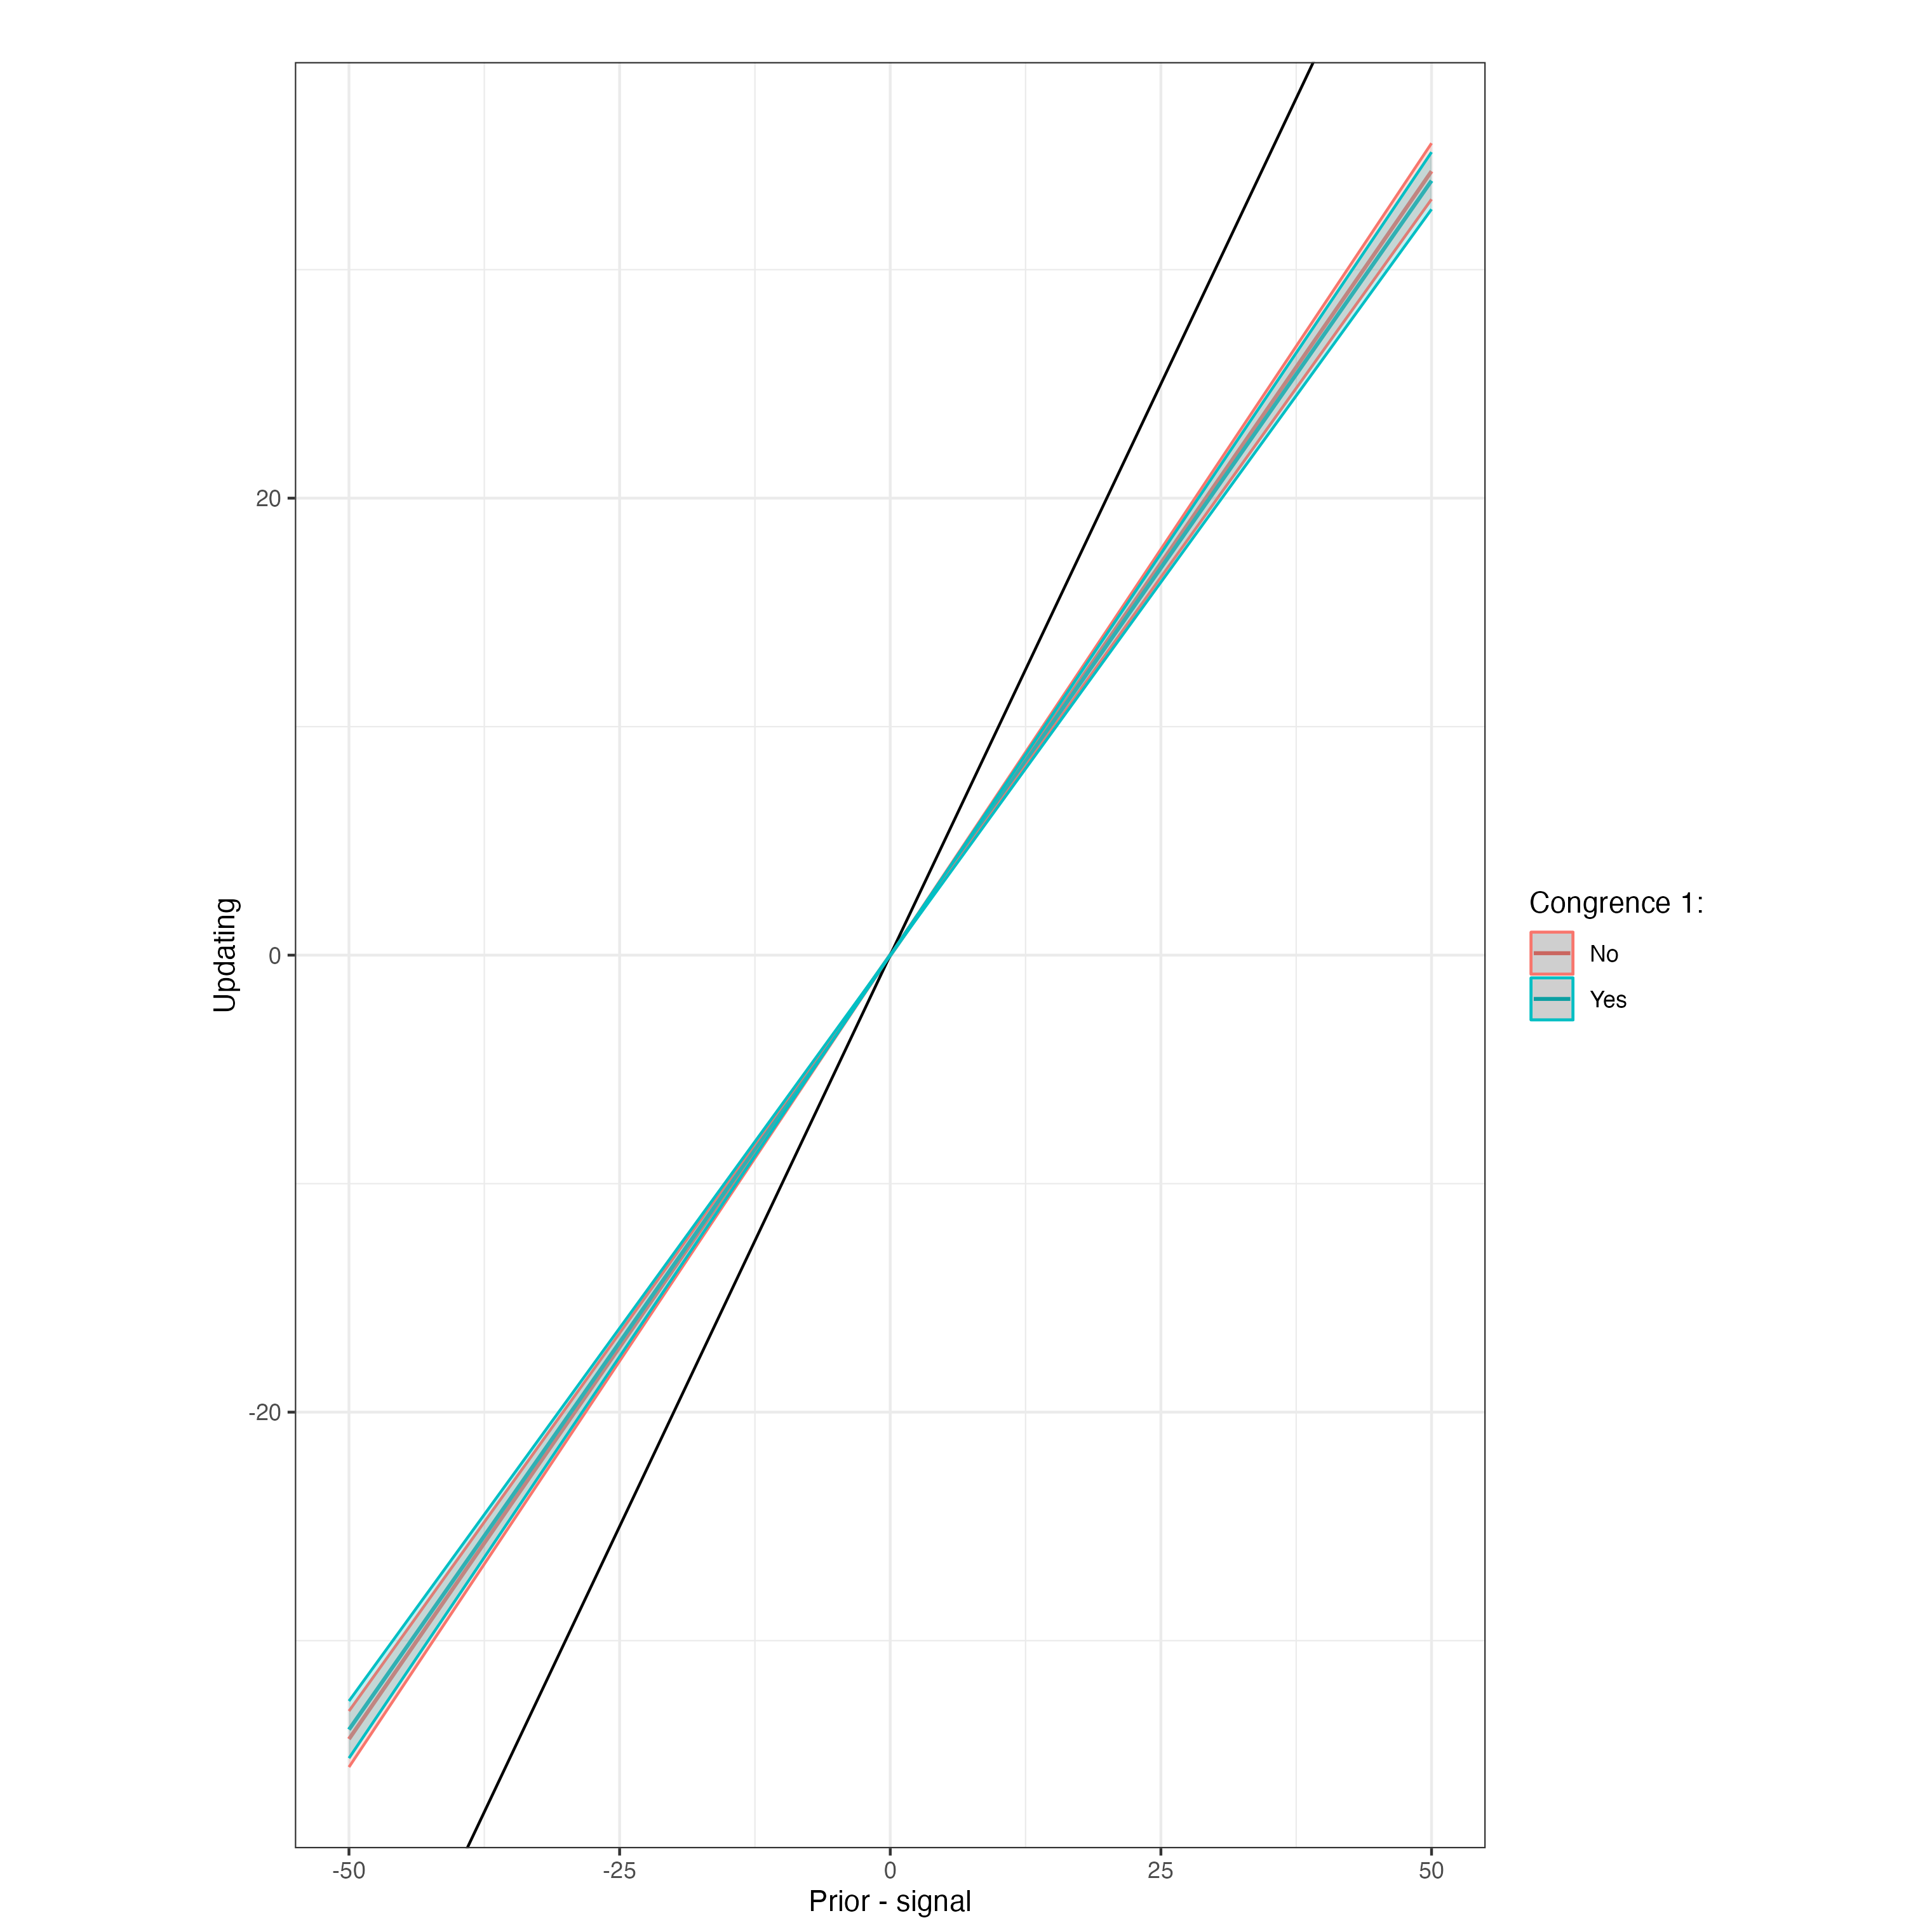
\includegraphics[height=8cm]{output/MainII_1.png}	
}
\only<2>{
\centering
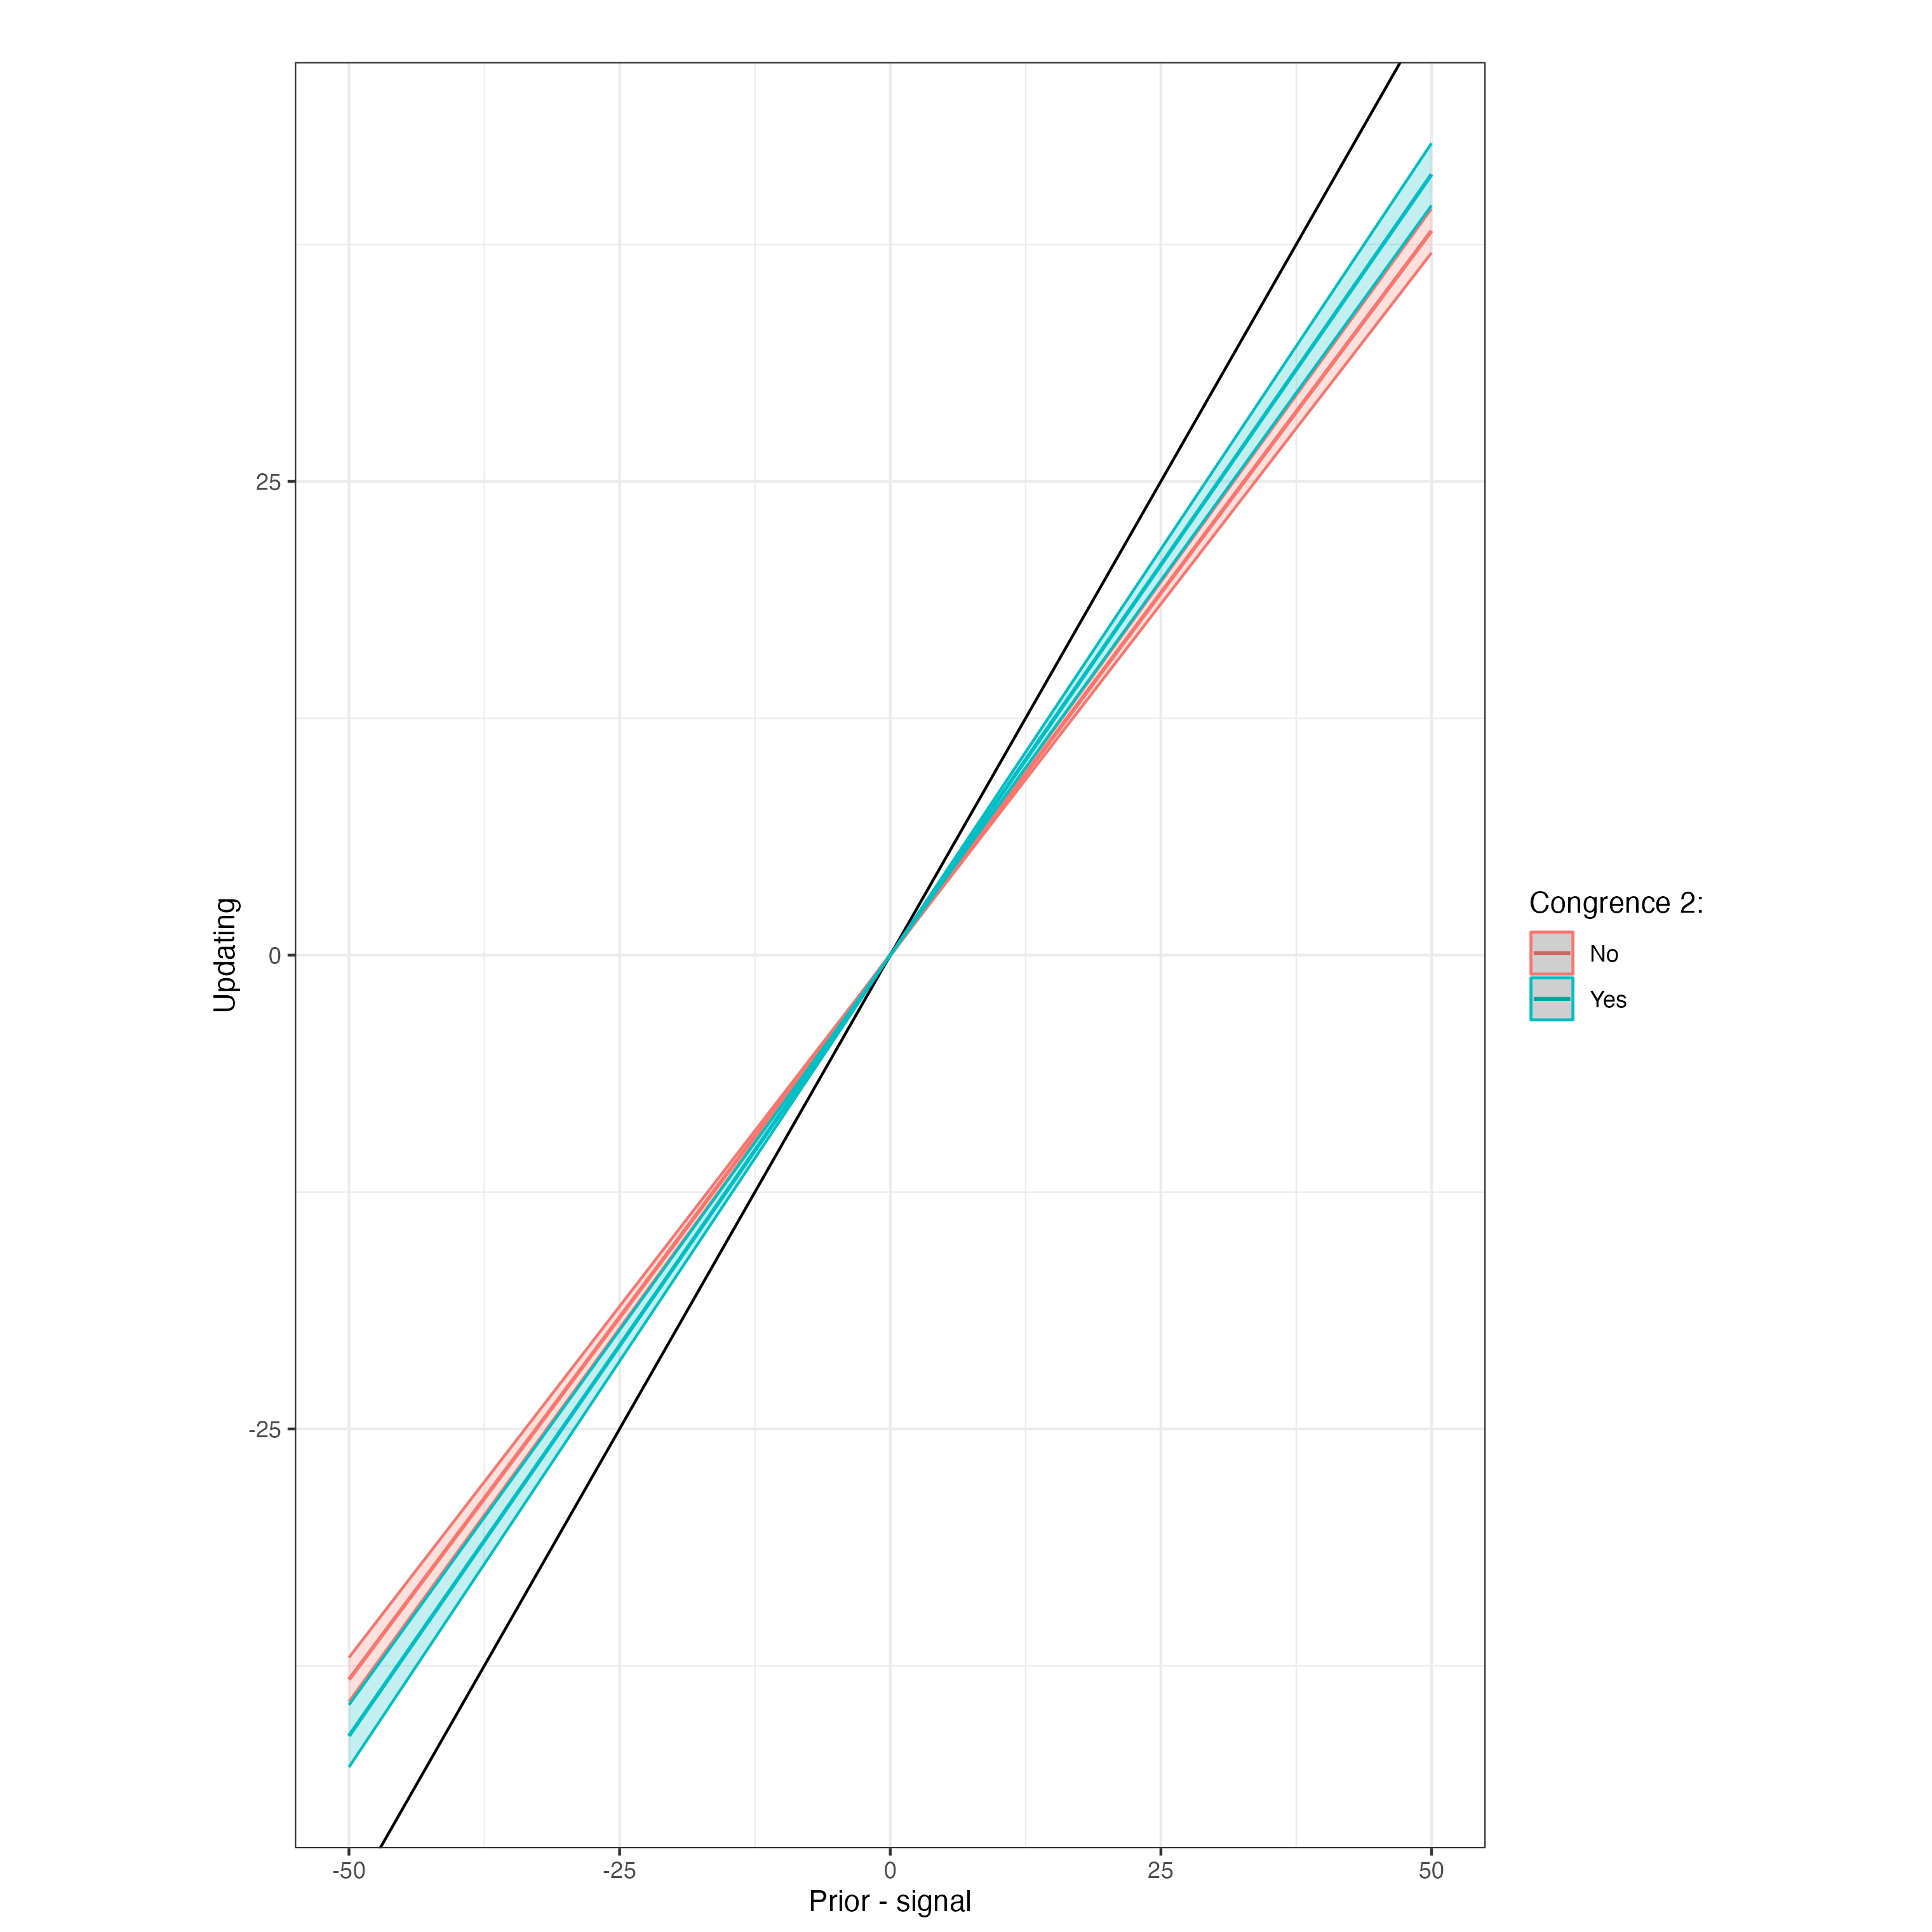
\includegraphics[height=8cm]{output/MainII_2.png}	
}
\only<3>{
\centering
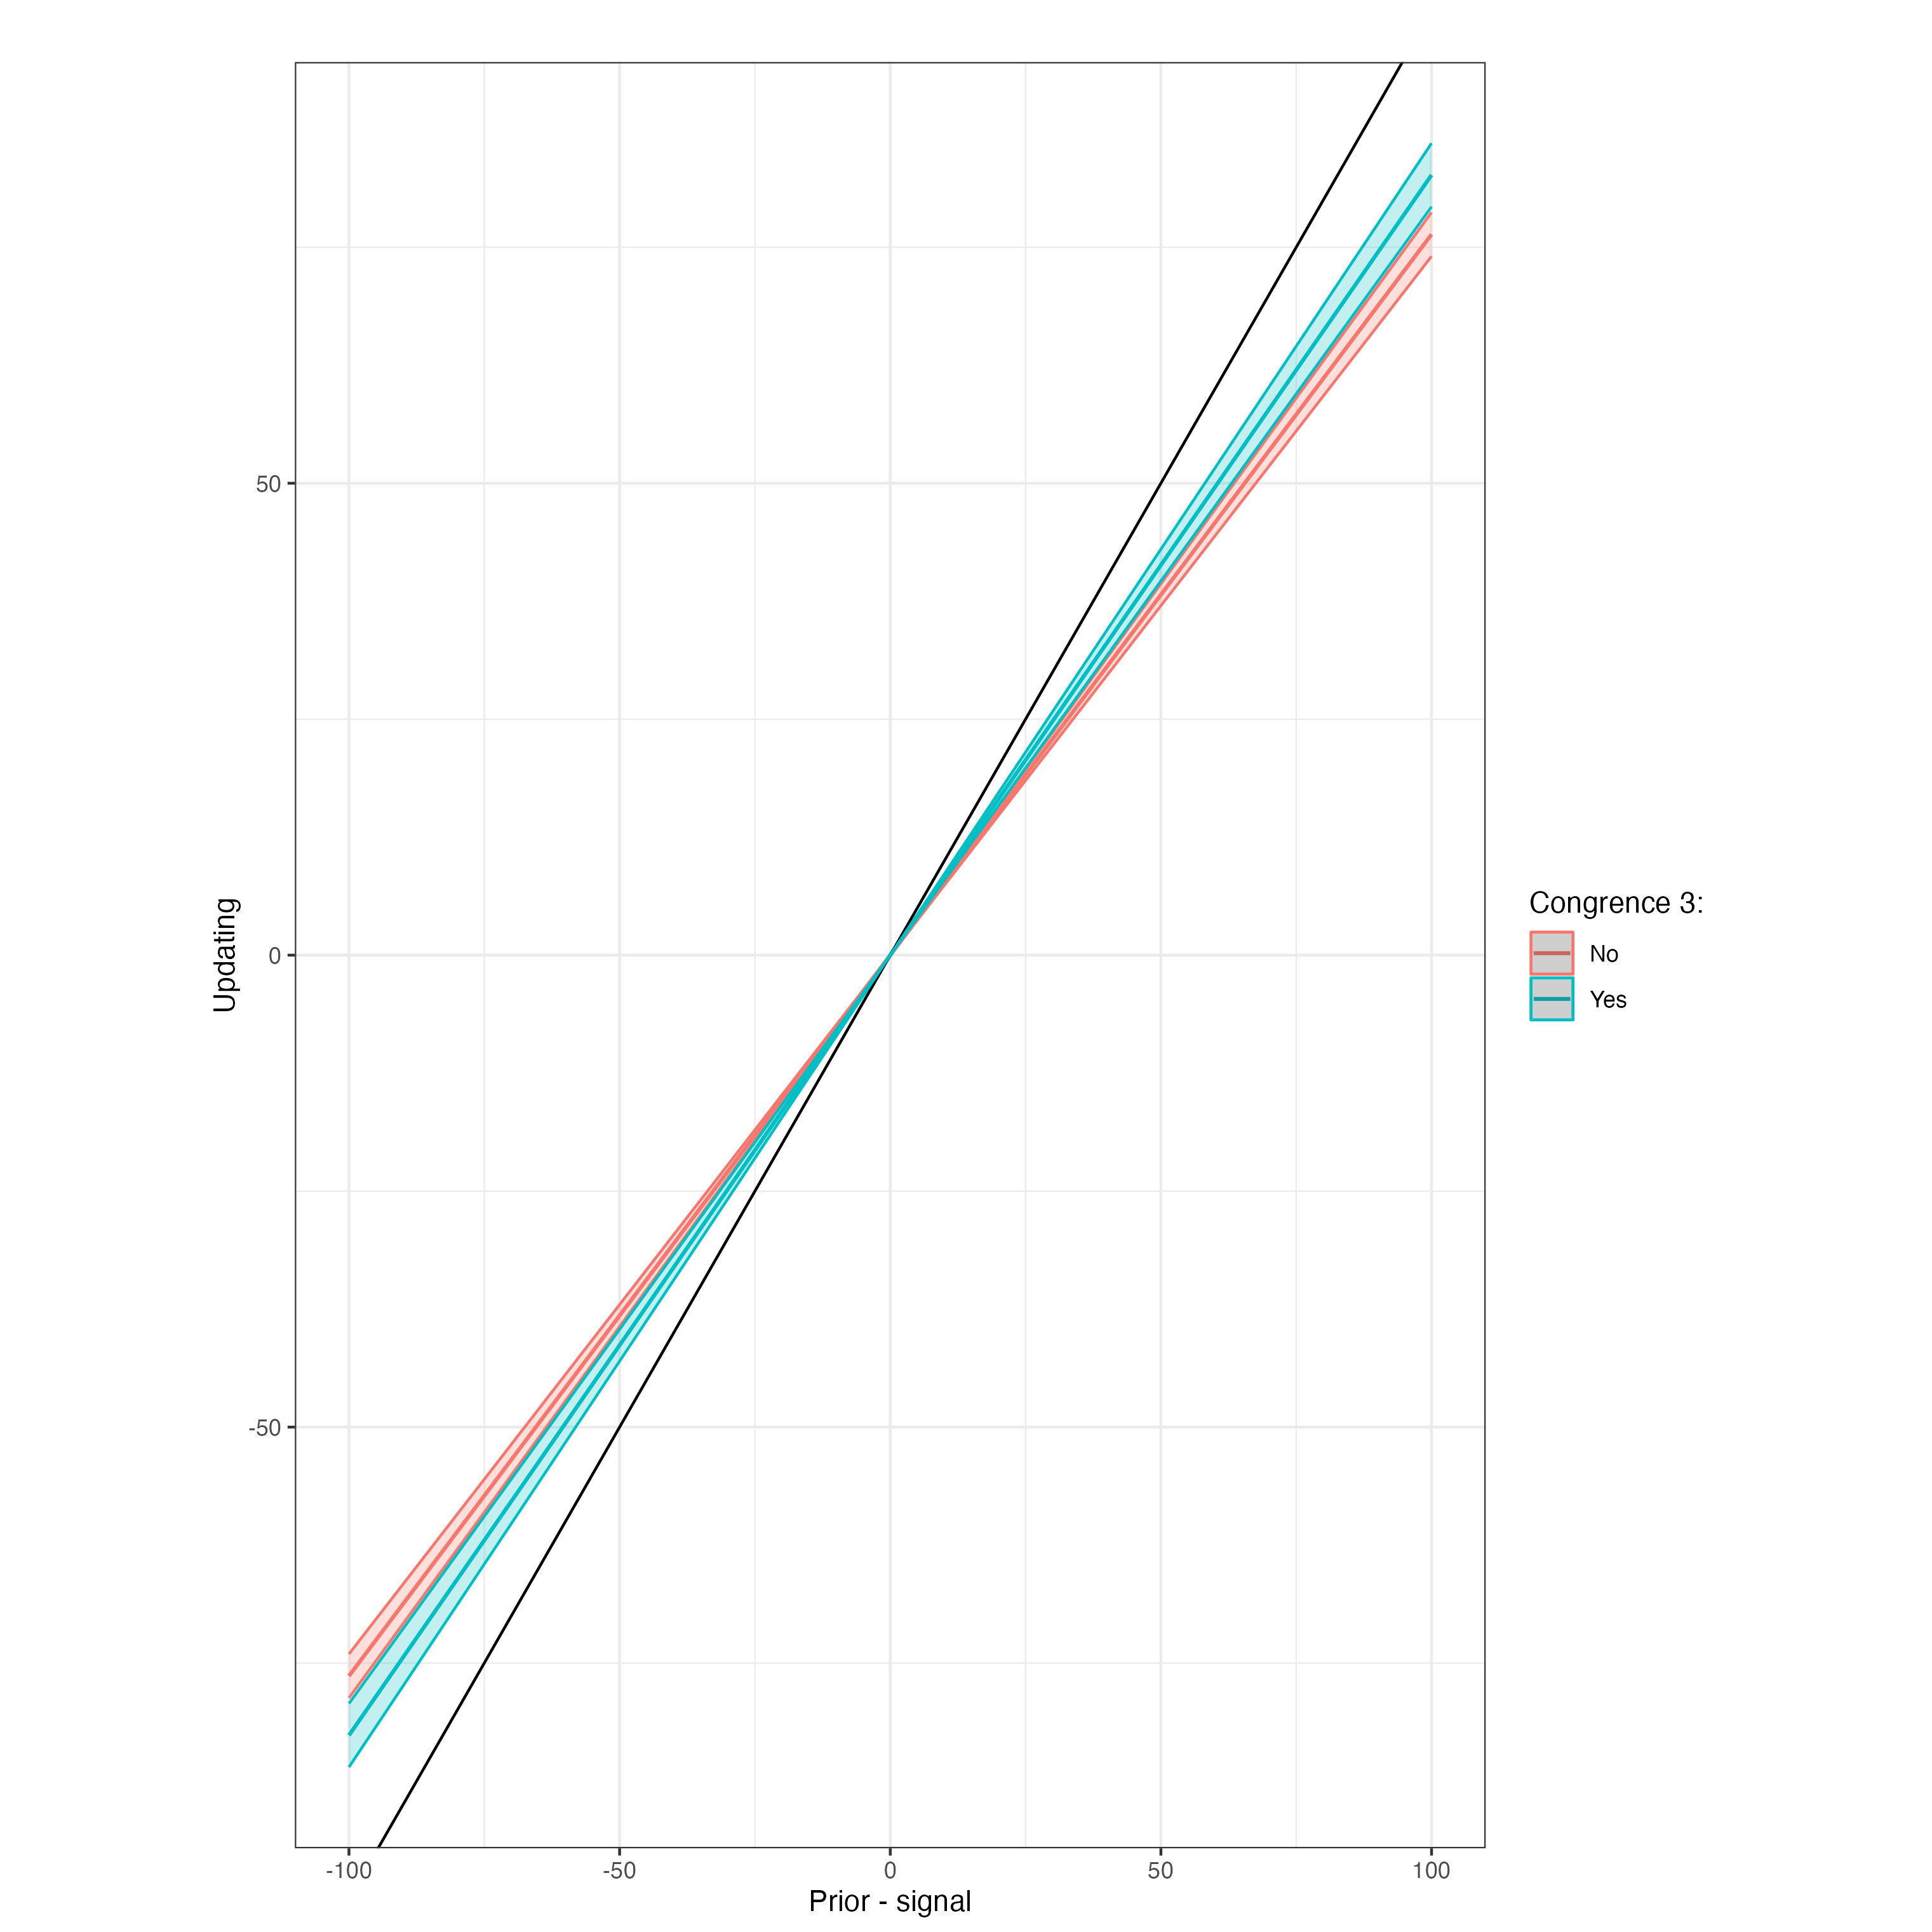
\includegraphics[height=8cm]{output/MainII_3.png}	
}
\column{0.35\textwidth}
\begin{itemize}
\only<1>{\item Congruence 1: \\ $\Delta$ slope = -0.008}
\item No significant effect on learning rates when presenter share's race with respondent
\only<2>{\item Congruence 2: \\ $\Delta$ slope = $0.060^{***}$}
\only<2->{\item 7.32\% better learning when information = audience
}
\only<3>{
\item Congruence 3: \\ $\Delta$ slope = $0.063^{***}$
}
\only<3->{
\item 7.7\% better learning when information = audience
}
\end{itemize}
\end{columns}
\vspace{-0.5cm}
  \hfill \hyperlink{mainII_reg}{\beamerbutton{Reg}}  
\end{frame}

\begin{frame}{Trust?}
\begin{itemize}
    \item Can the results be explained by differences in trust?
    \item Subjective posterior: what respondents think you actual number is, not necessarily the one in the video
    \item Heterogeneity analysis based on whether they reported a different subjective posterior than signal
\end{itemize}
\end{frame}


\begin{frame}{Trust does not change the role of congruence}
\only<1>{
\begin{adjustbox}{width=\textwidth, totalheight=\textheight-\baselineskip,keepaspectratio}
\begin{threeparttable}
\begin{tabular}[t]{lccc}
\toprule
  & Presenter/Audience & Audience/Info & Presenter/Info\\
\addlinespace[0.5em]
\midrule \hspace{1em}Congruence & -0.031 & -1.355*** & -1.474***\\
\hspace{1em} & (0.371) & (0.236) & (0.238)\\
\hspace{1em}Different posterior & 3.269*** & 3.209*** & 2.962***\\
\hspace{1em} & (0.455) & (0.453) & (0.444)\\
\hspace{1em}Congruence $\times$ Different posterior & 0.298 & -0.435 & 0.412\\
\hspace{1em} & (0.639) & (0.513) & (0.514)\\
\hspace{1em}Black stratum & 4.350*** & 2.656*** & 2.656***\\
\hspace{1em} & (0.335) & (0.423) & (0.423)\\
\hspace{1em}Black presenter &  & 0.037 & 0.036\\
\hspace{1em} &  & (0.413) & (0.413)\\
\hspace{1em}Constant & 9.310*** & 10.404*** & 10.440***\\
\hspace{1em} & (0.781) & (0.946) & (0.944)\\
\hspace{1em}Adj.R$2$ & 0.04 & 0.04 & 0.04\\
\addlinespace[0.5em]
\midrule
\hspace{1em}N & 16909 & 7519 & 7519\\
\bottomrule
\multicolumn{4}{l}{\rule{0pt}{1em}* p $<$ 0.05, ** p $<$ 0.01, *** p $<$ 0.001}\\
\end{tabular}
\begin{tablenotes}[para]
\item \textit{Note: } 
\item Standard errors in parenthesis are clustered at the individual level.
      Observations are at the individual-fact level. 
\end{tablenotes}
\end{threeparttable}
\end{adjustbox}
}
\only<2>{
\begin{adjustbox}{width=\textwidth, totalheight=\textheight-\baselineskip,keepaspectratio}
\begin{threeparttable}
\begin{tabular}[t]{lccc}
\toprule
  & Presenter/Audience & Audience/Info & Presenter/Info\\
\addlinespace[0.5em]
\midrule \hspace{1em}Signal - prior & 0.788*** & 0.741*** & 0.737***\\
\hspace{1em} & (0.041) & (0.052) & (0.051)\\
\hspace{1em}$(s - pr) \times$ Congruence & 0.004 & 0.055** & 0.071***\\
\hspace{1em} & (0.020) & (0.018) & (0.018)\\
\hspace{1em}$(s - pr) \times$  Different posterior & -0.086*** & -0.072** & -0.067**\\
\hspace{1em} & (0.024) & (0.024) & (0.024)\\
\hspace{1em}$(s - pr) \times$ Congruence $\times$ Different posterior & -0.043 & 0.013 & -0.014\\
\hspace{1em} & (0.034) & (0.035) & (0.036)\\
\hspace{1em}$(s - pr) \times$ Black stratum & -0.154*** & -0.109*** & -0.105***\\
\hspace{1em} & (0.018) & (0.024) & (0.024)\\
\hspace{1em}$(s - pr) \times$ Black presenter &  & 0.006 & 0.002\\
\hspace{1em} &  & (0.023) & (0.023)\\
\hspace{1em}Adj.R$2$ & 0.47 & 0.63 & 0.63\\
\midrule
\hspace{1em}N & 16909 & 7519 & 7519\\
\bottomrule
\multicolumn{4}{l}{\rule{0pt}{1em}* p $<$ 0.05, ** p $<$ 0.01, *** p $<$ 0.001}\\
\end{tabular}
\begin{tablenotes}[para]
\item \textit{Note: } 
\item Standard errors in parenthesis are clustered at the individual level.
      Observations are at the individual-fact level. 
\end{tablenotes}
\end{threeparttable}
\end{adjustbox}
}
% $Different posterior$ is a dummy variable indicating whether the respondents indicated a different \texit{subjective} posterior than the signal.
\end{frame}




\section{Conclusion}


\begin{frame}{Conclusion}
\begin{block}{Today}
\begin{itemize}
    \item Incentivized information provision experiment to study role of congruence in identity between components of communication
    \begin{itemize}
    \item Individuals learn better information that regard their own group, or when presented by someone belonging to that group
    \item Individuals do not learn better information when presented by someone from their own group
    \item Monetary incentives do not play a role, neither trust
    \end{itemize}
    \item Methodology is quite “portable”
\end{itemize}
\end{block}
\begin{block}{Avenues for future research }
\begin{itemize}
    \item Why?
    \begin{itemize}
    \item Congruence 1 : Salience of presenter's identity
    \item Congruence 2 : Correlation between congruence 2 and implicit bias 
    \item Congruence 3 : Complementary in salience
    \end{itemize}
    \item Use other social identity groups: e.g. political affiliation, gender, etc.
\end{itemize}
\end{block}
\end{frame}



\begin{frame}[standout]
Thank you!\\
\vspace{1cm}
\large{\url{luisa.carrer@uzh.ch}}

\end{frame}

\appendix
{\metroset{background=dark}
\begin{frame}{}
    Appendix
\end{frame}
}


{\setbeamercolor{frametitle}{fg=palette primary, bg=palette primary}
\begin{frame}{All Pictures}
\label{all_pic}
\begin{adjustwidth}
\vspace{-1.5cm}
\hfill \hyperlink{pic examples}{\beamerbutton{Back}}
\vspace{-1cm}
\begin{figure}[h!]
\centering
\hspace{0.485\textwidth}
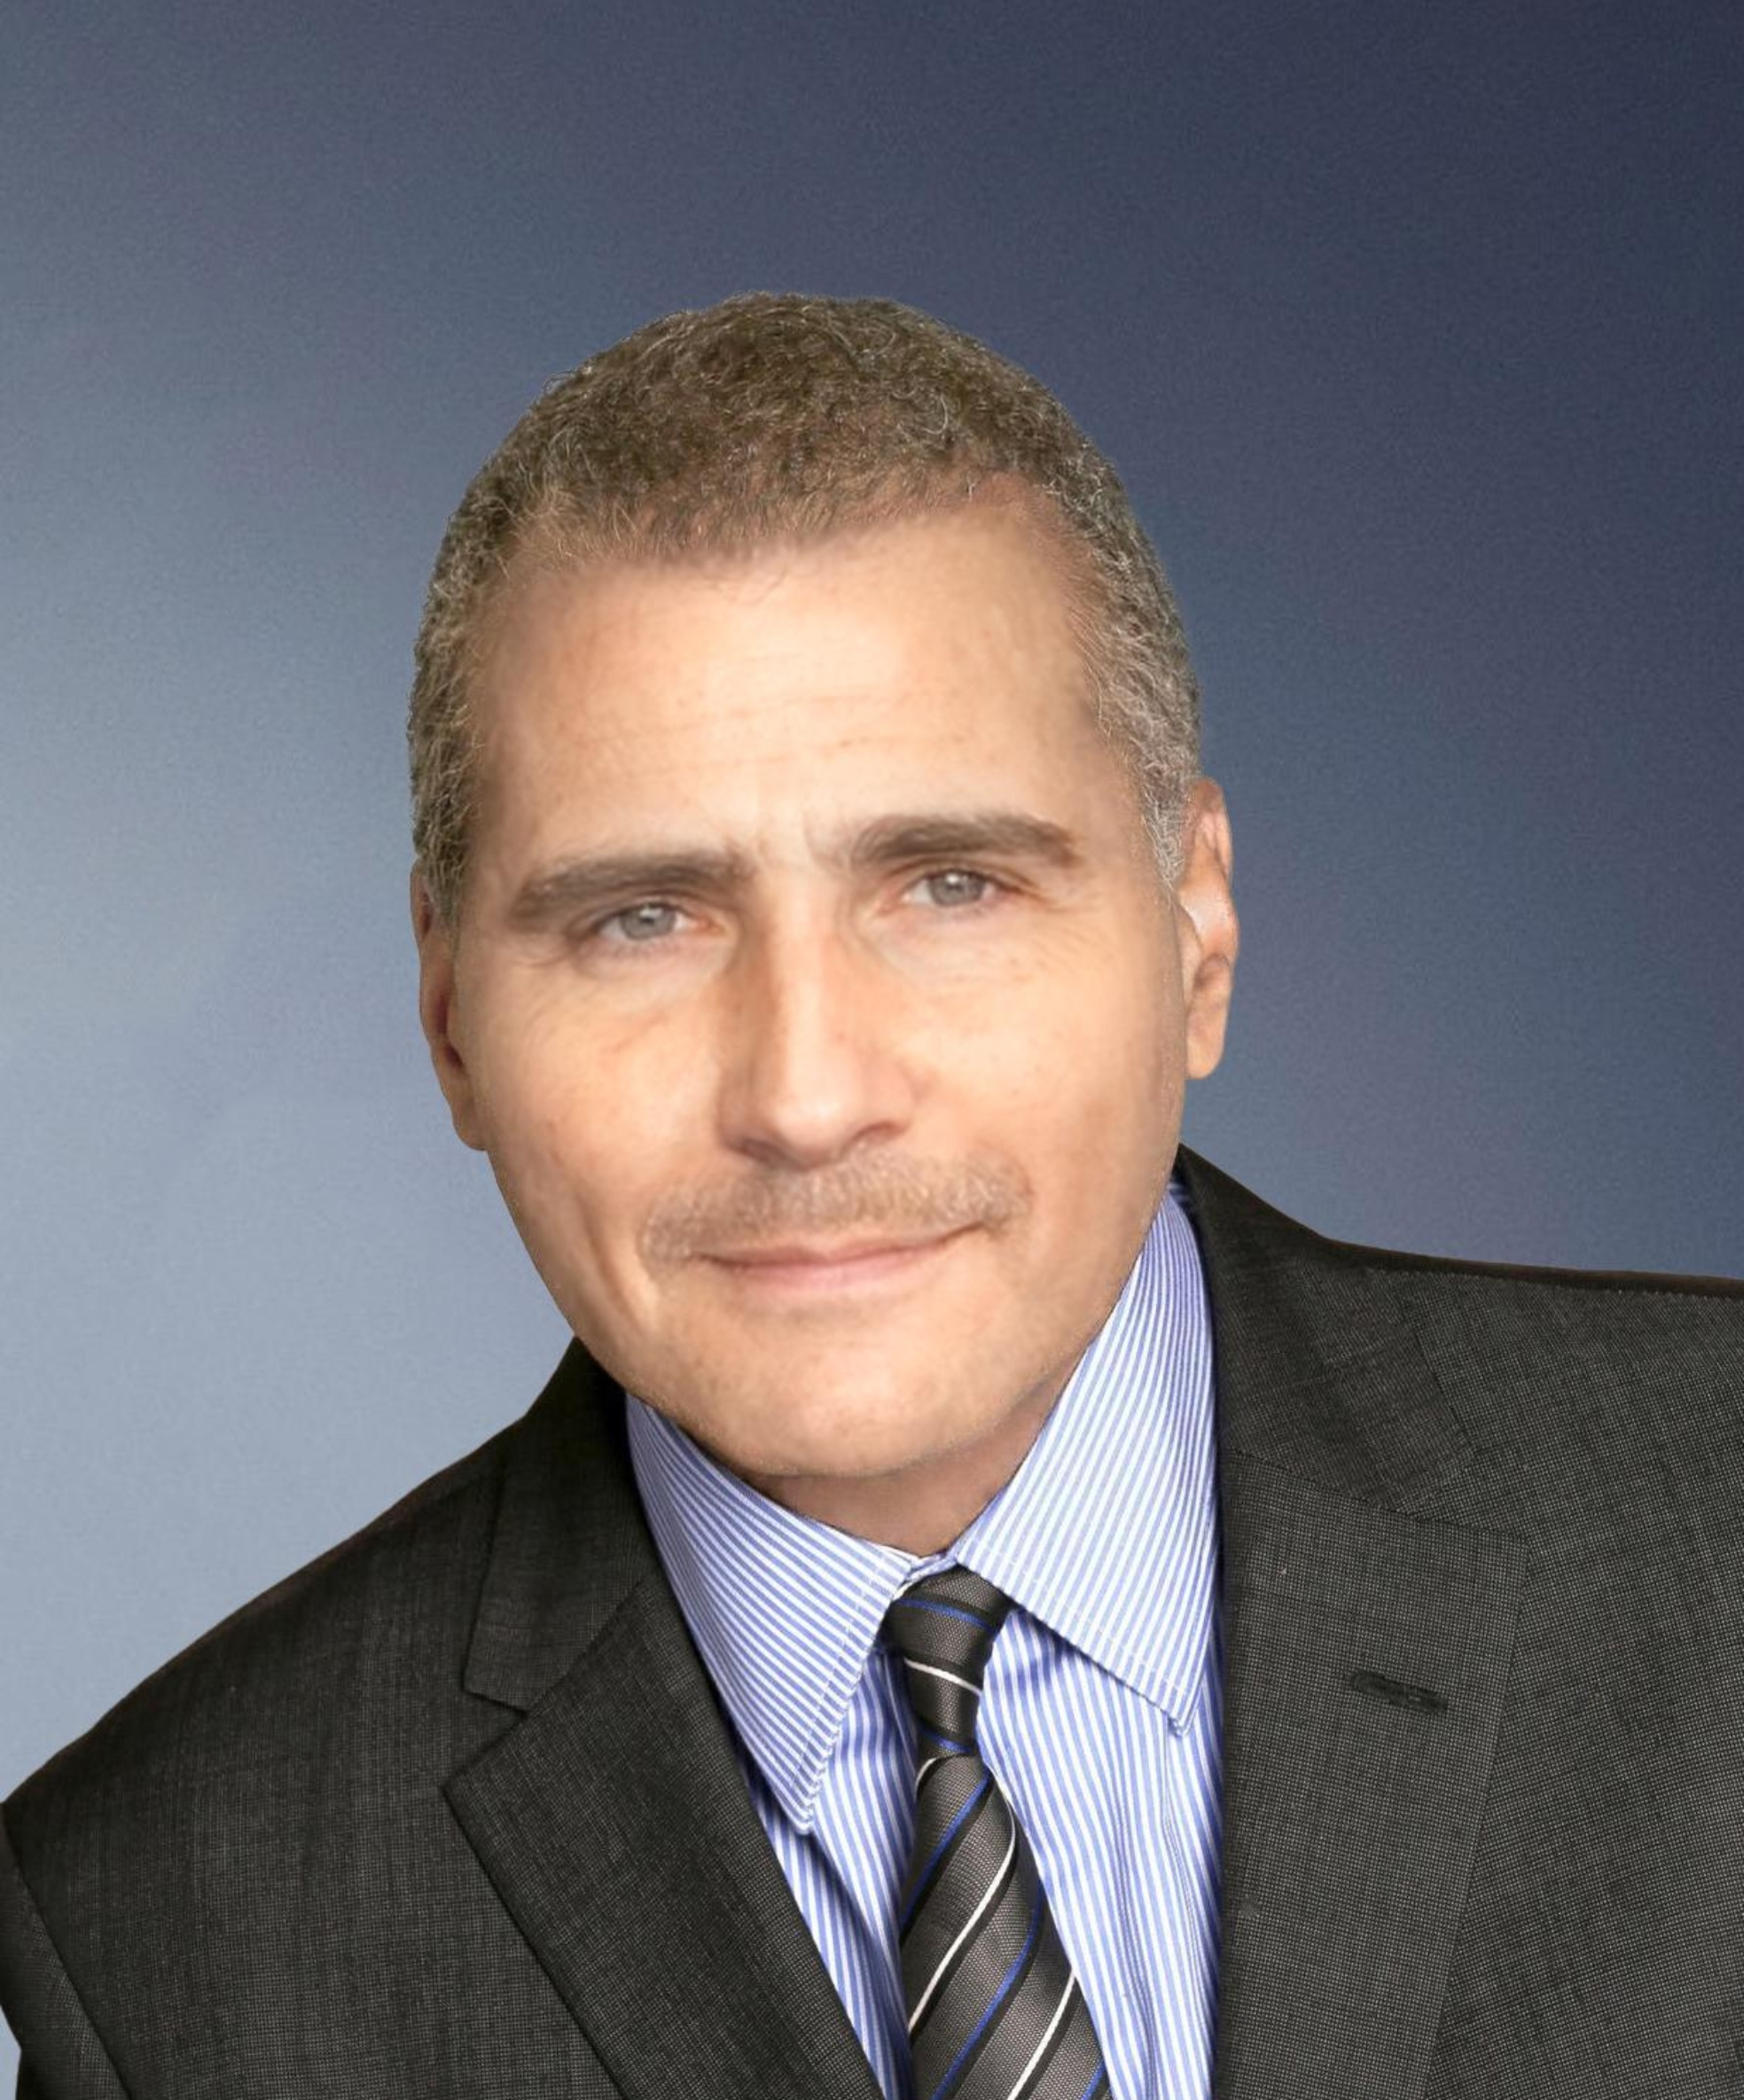
\includegraphics[width=0.11\textwidth]{img/pic/whitakerBLUE-WM-221.jpg}\hspace{0.1em}
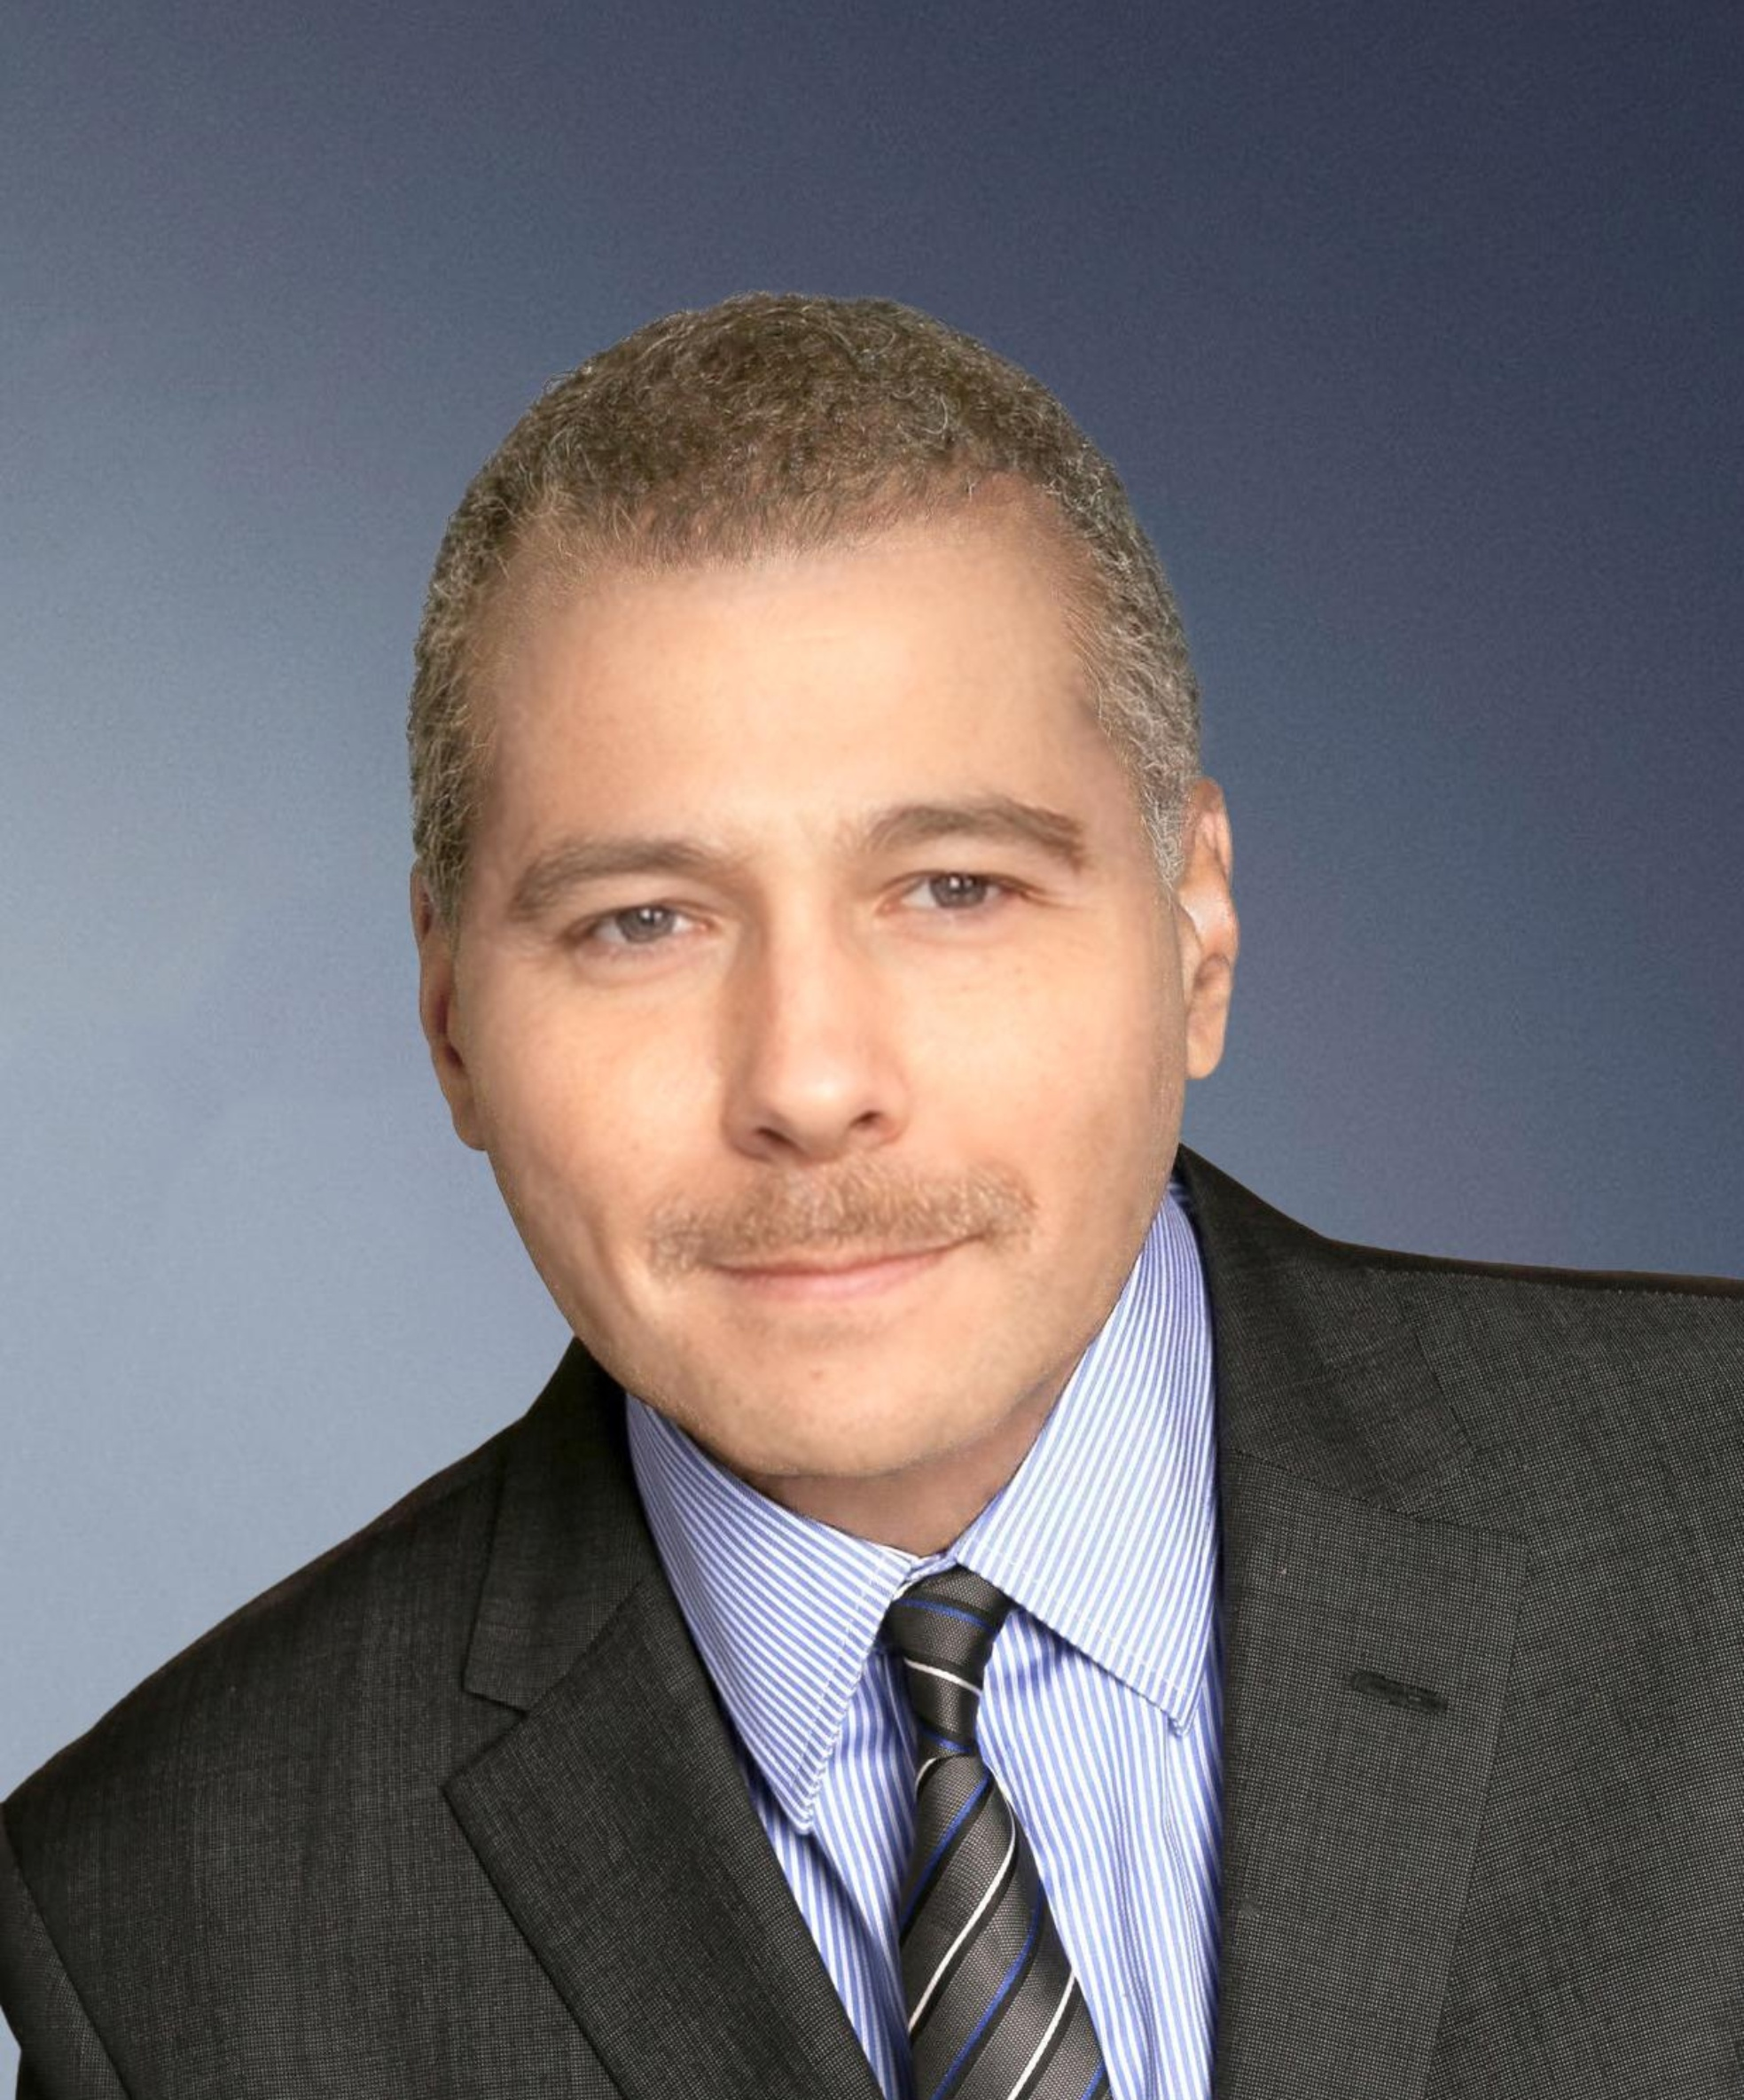
\includegraphics[width=0.11\textwidth]{img/pic/whitakerBLUE-WM-214.jpg}\hspace{0.1em}
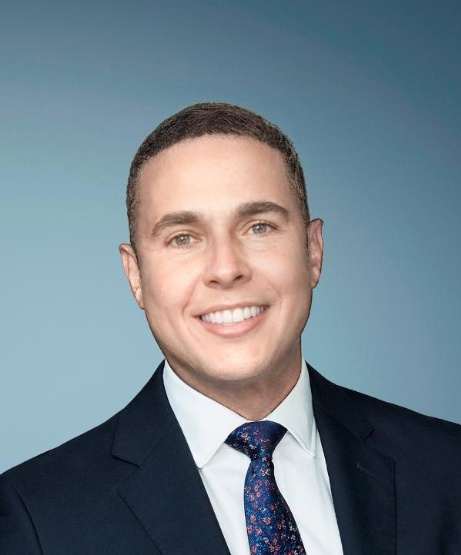
\includegraphics[width=0.11\textwidth]{img/pic/lemon-WM-241.jpg}
\\ 
\centering
\hspace{0.485\textwidth}
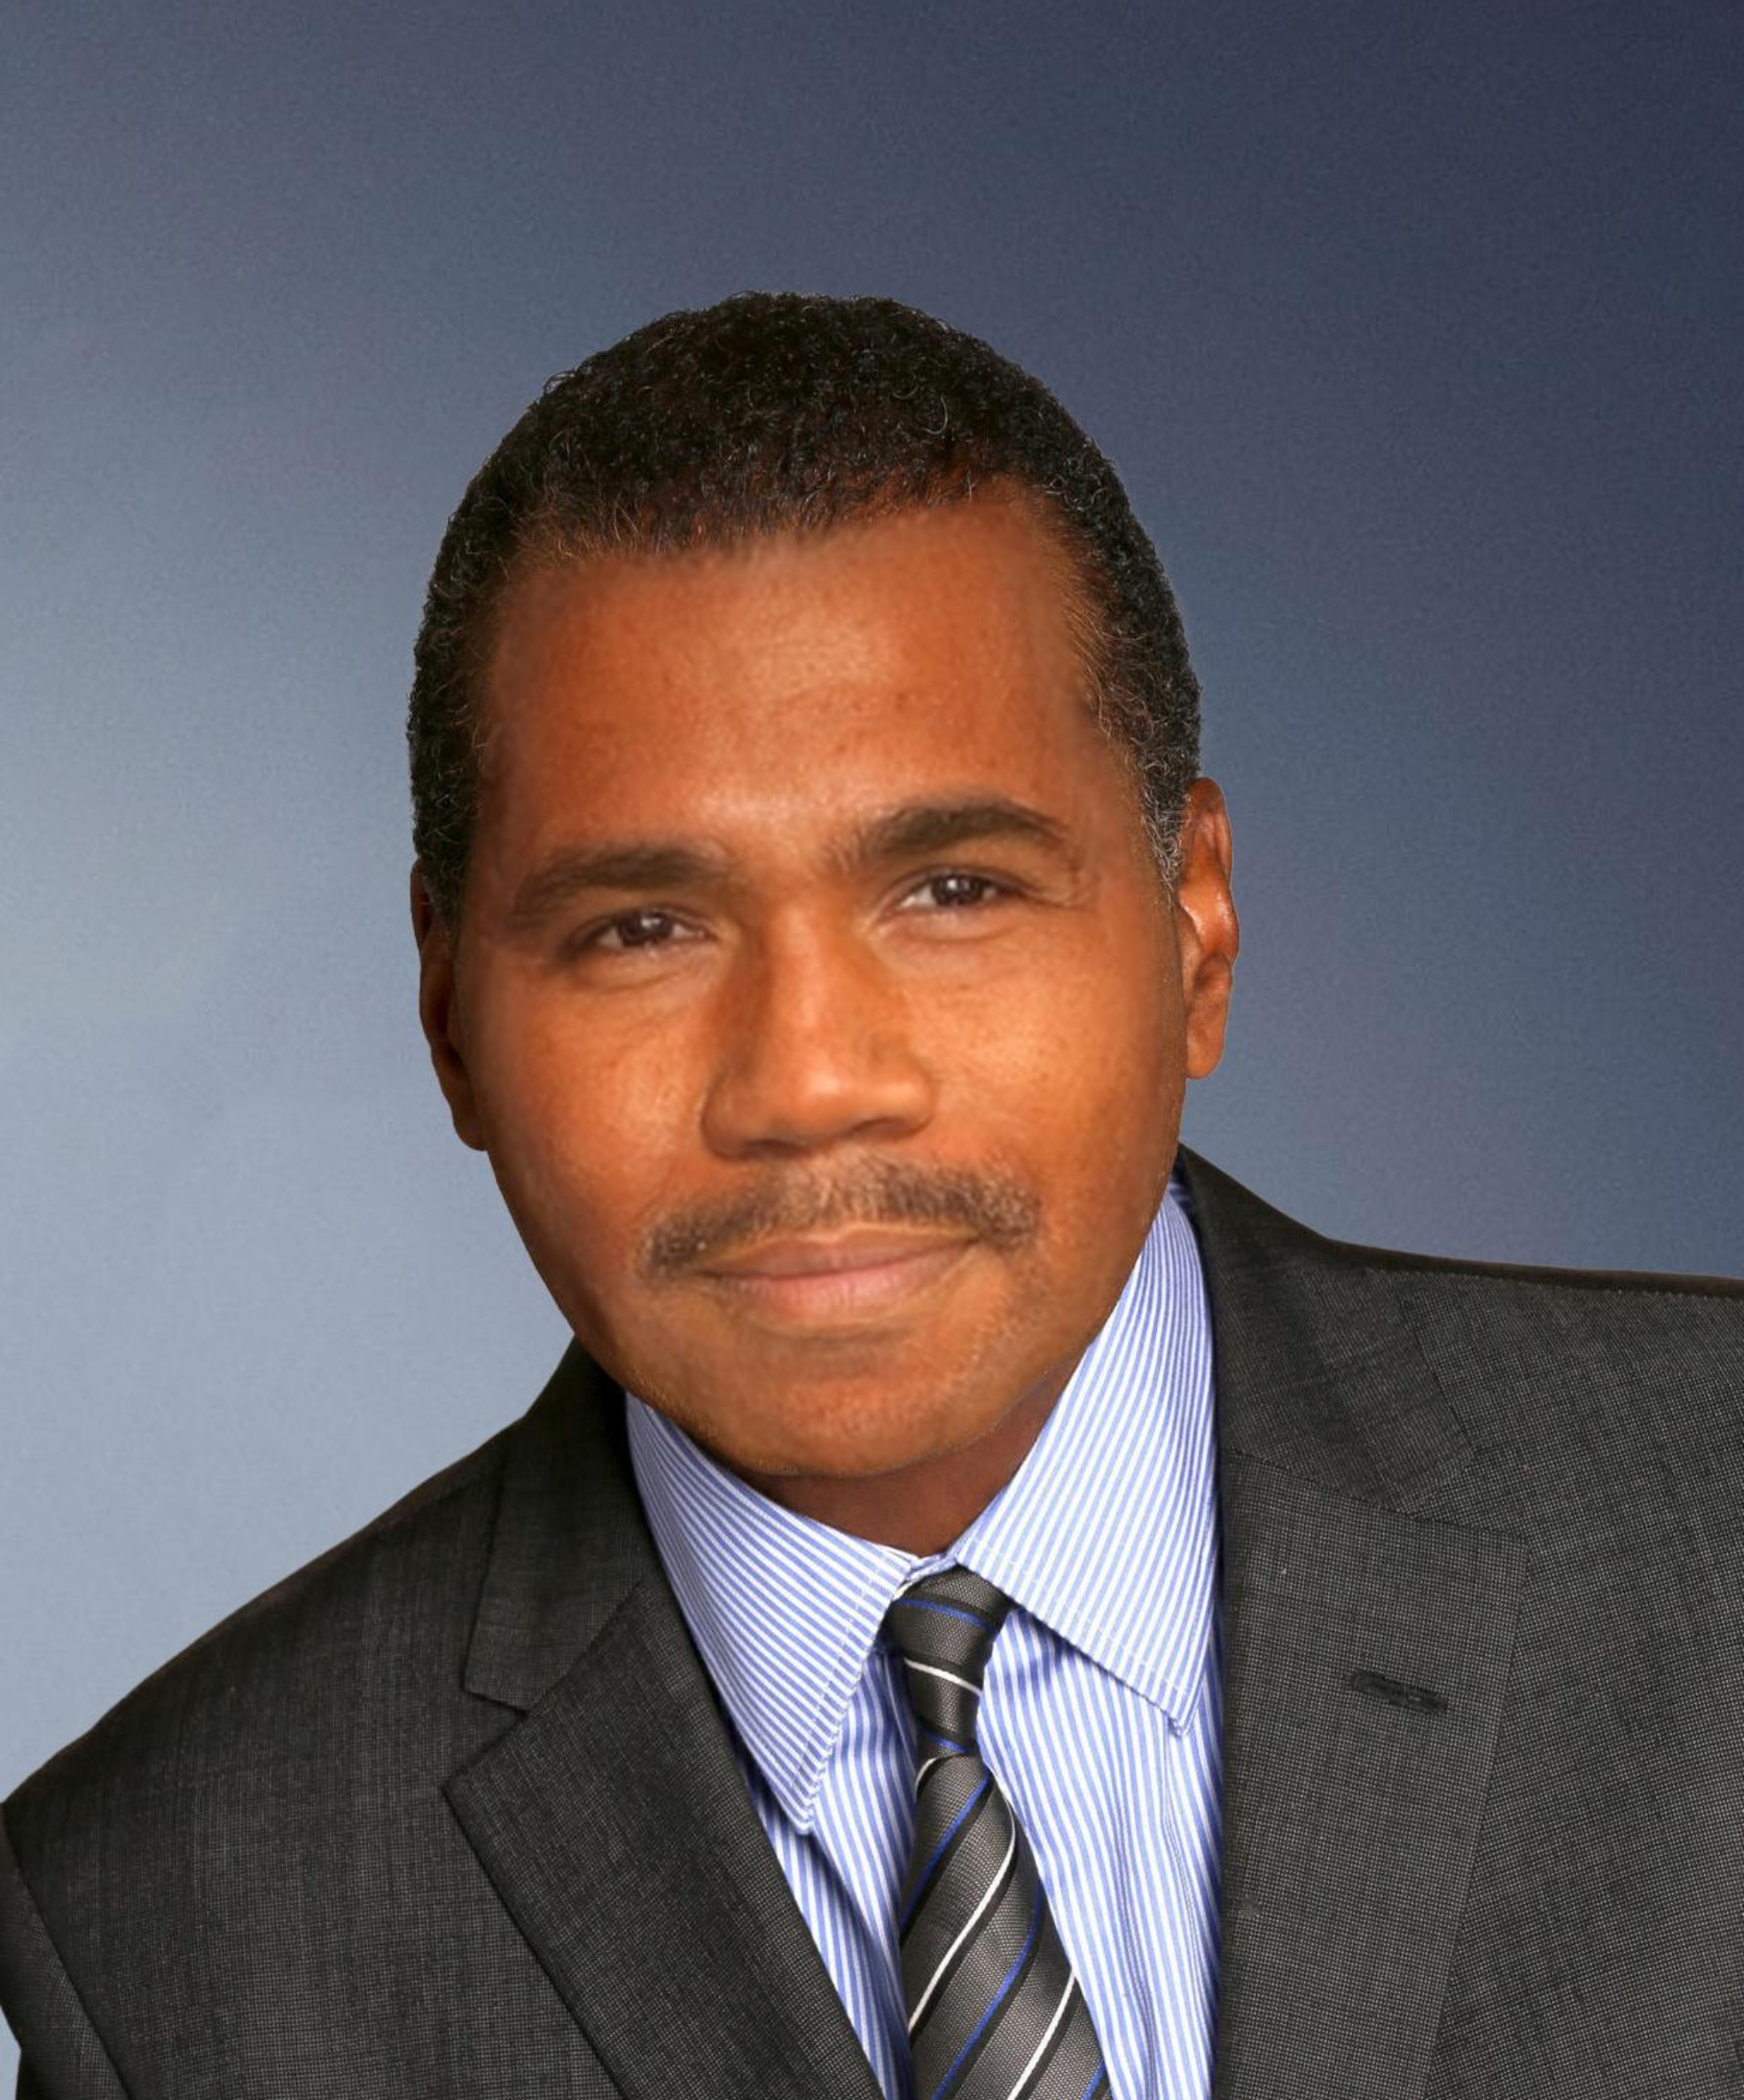
\includegraphics[width=0.11\textwidth]{img/pic/whitakerBLUE-BM-206.jpg}\hspace{0.1em}
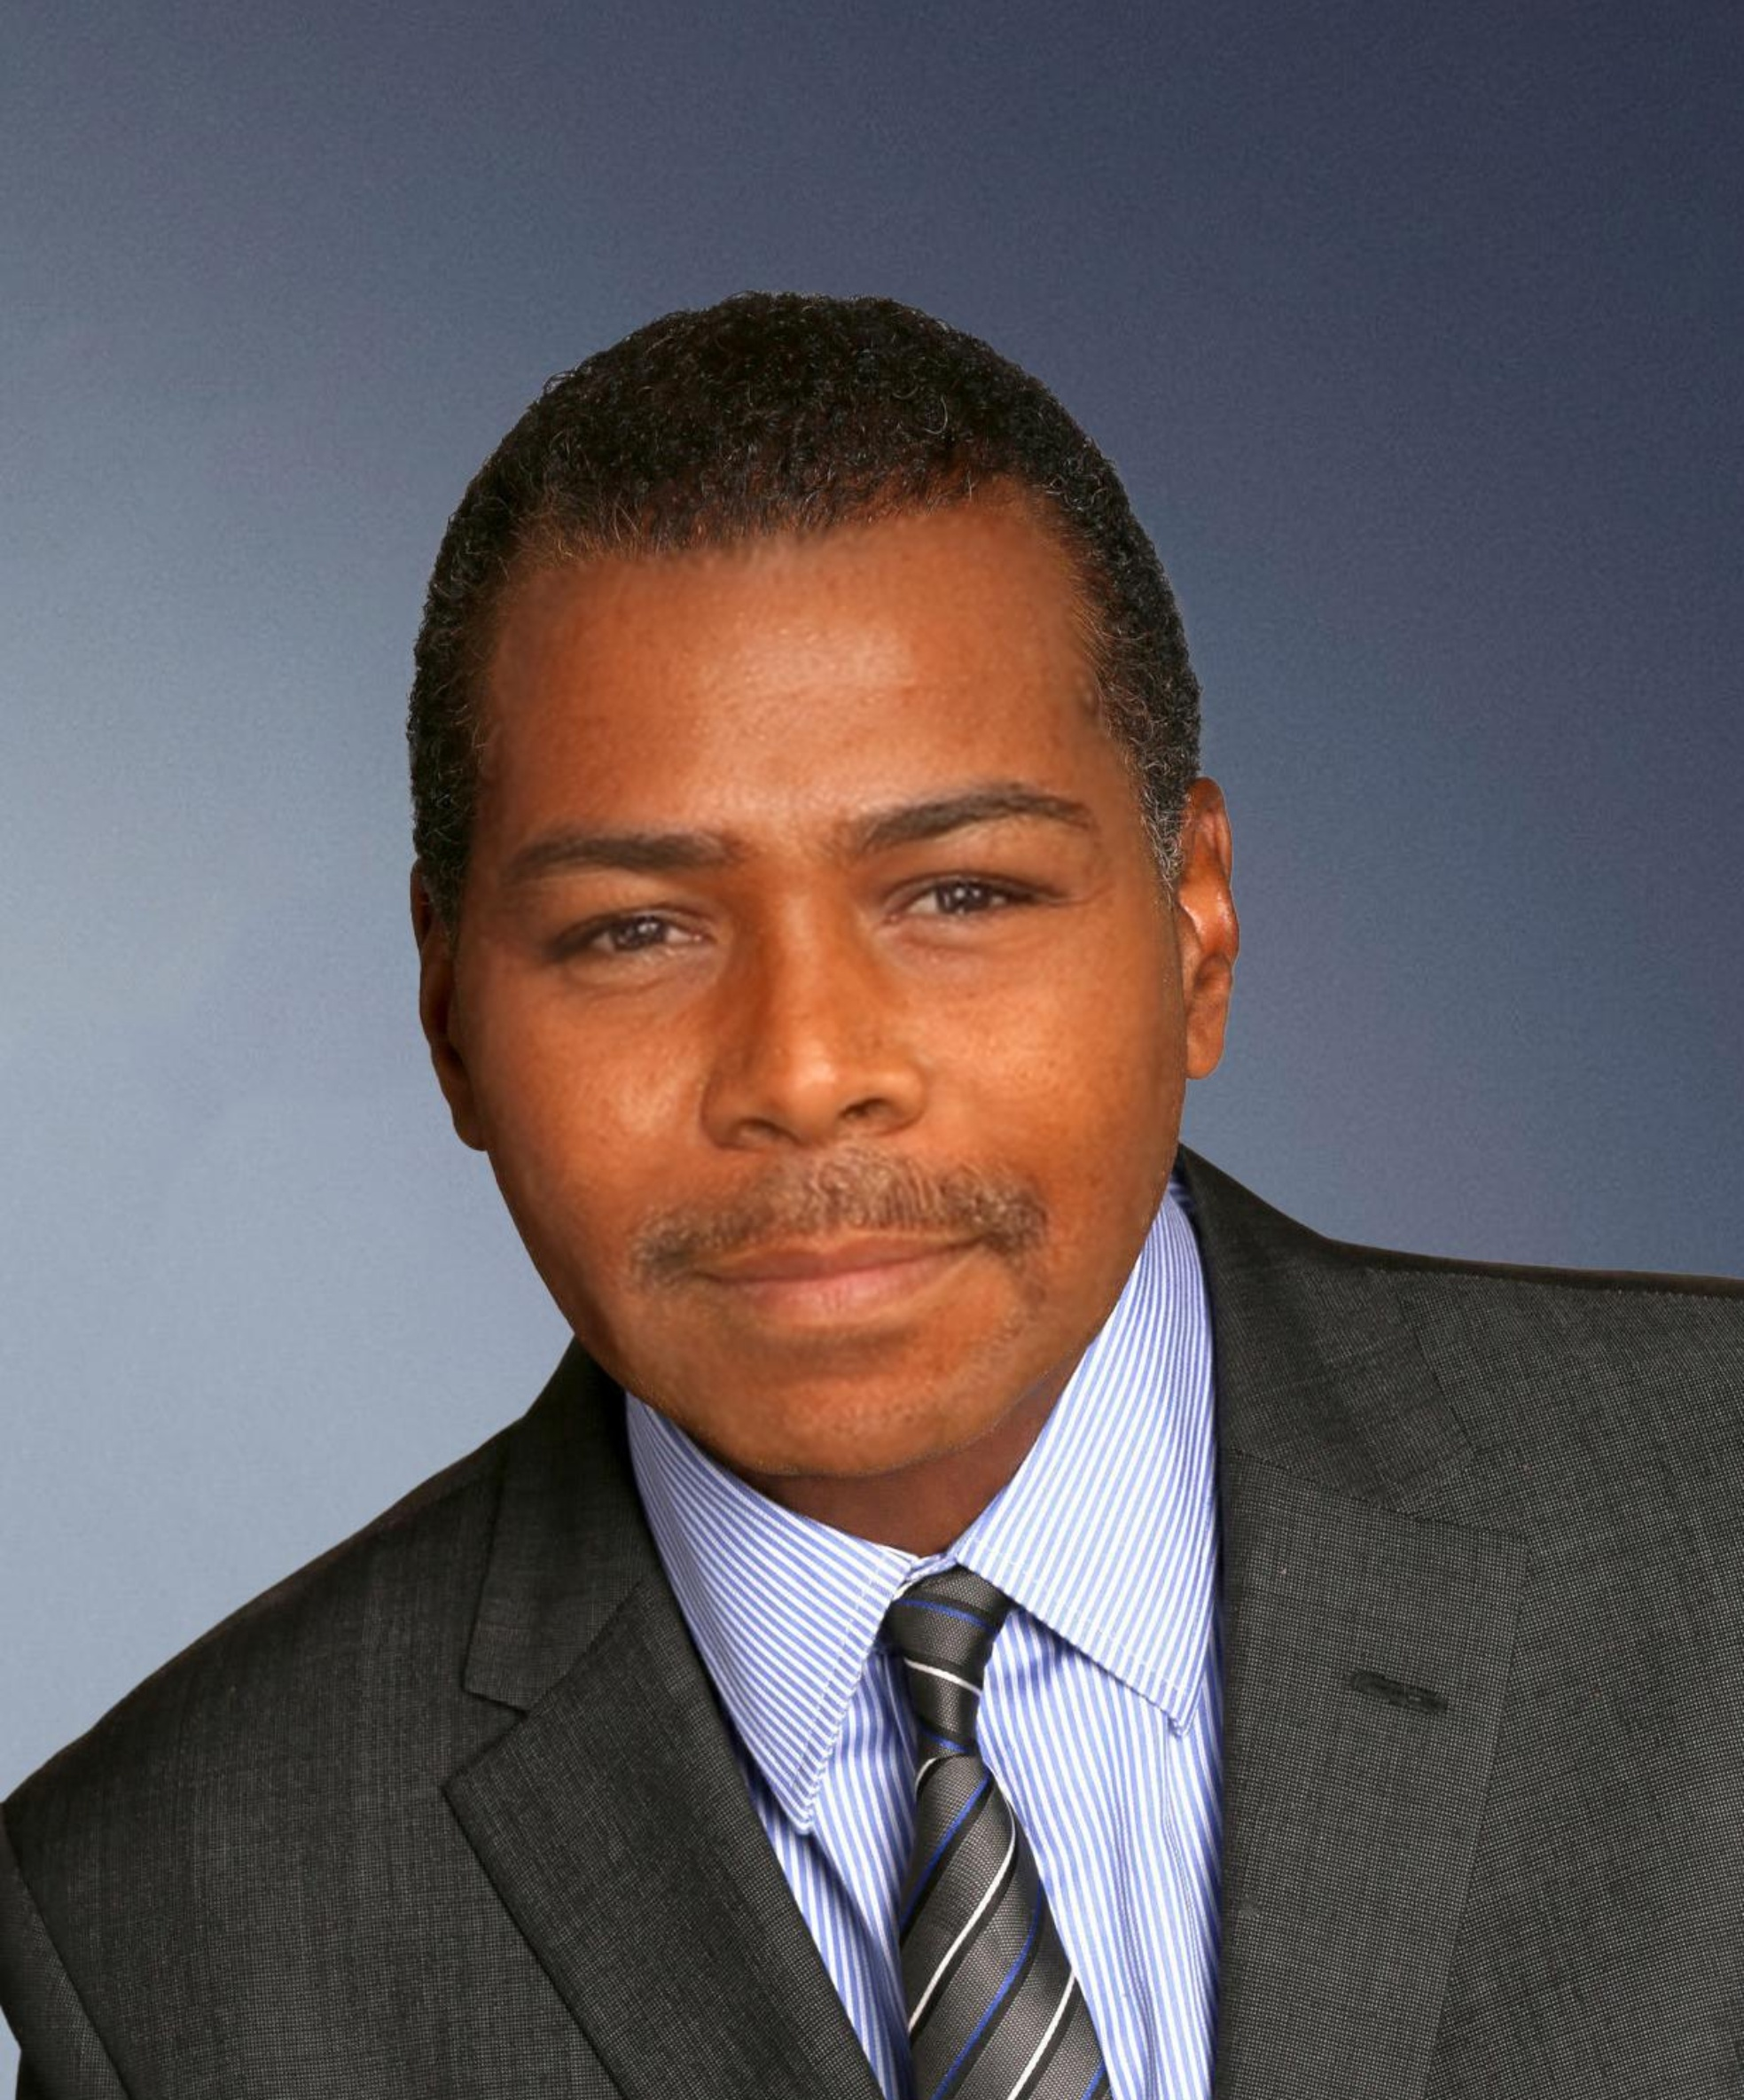
\includegraphics[width=0.11\textwidth]{img/pic/whitakerBLUE-BM-251.jpg}\hspace{0.1em}
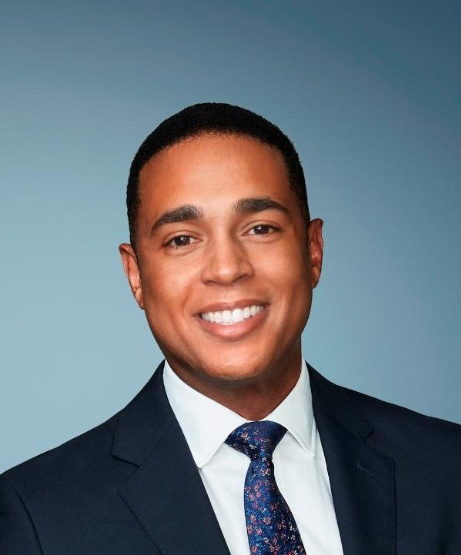
\includegraphics[width=0.11\textwidth]{img/pic/lemon-BM-204.jpg}\hfill
\\
   \centering

\includegraphics[width=0.11\textwidth]{img/pic/brunhuber-WM-026.jpg}\hfill

\includegraphics[width=0.11\textwidth]{img/pic/brunhuber-WM-249.jpg}\hfill

\includegraphics[width=0.11\textwidth]{img/pic/brunhuber-WM-241.jpg}\hfill
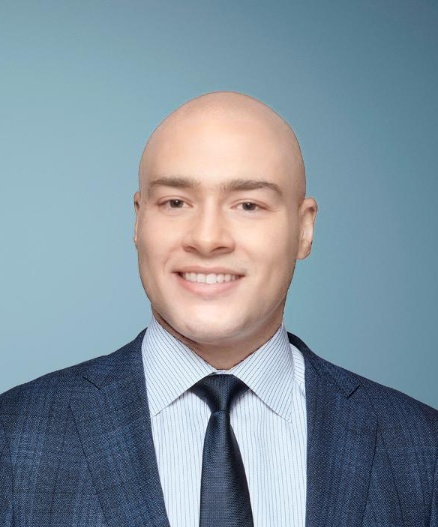
\includegraphics[width=0.11\textwidth]{img/pic/brunhuber-WM-242.jpg}\hfill
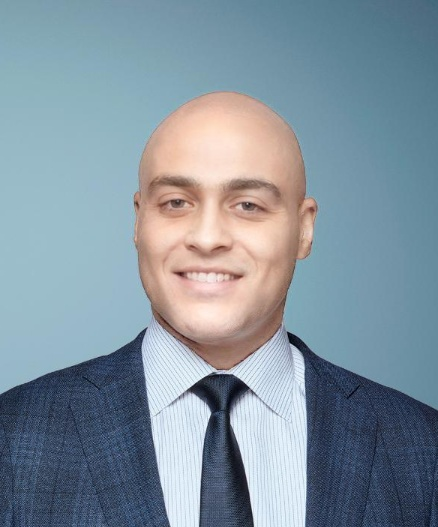
\includegraphics[width=0.11\textwidth]{img/pic/brunhuber-WM-243.jpg}\hfill
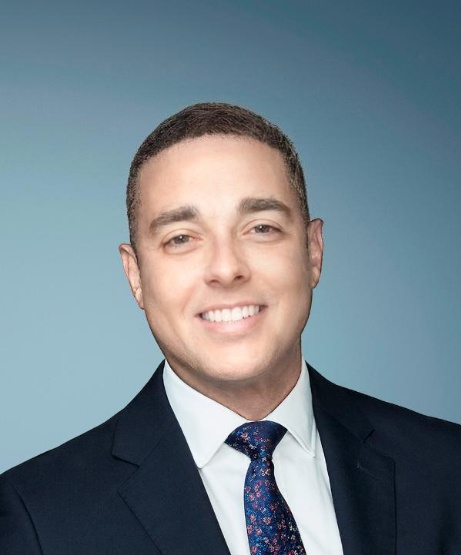
\includegraphics[width=0.11\textwidth]{img/pic/lemon-WM-023.jpg}\hfill
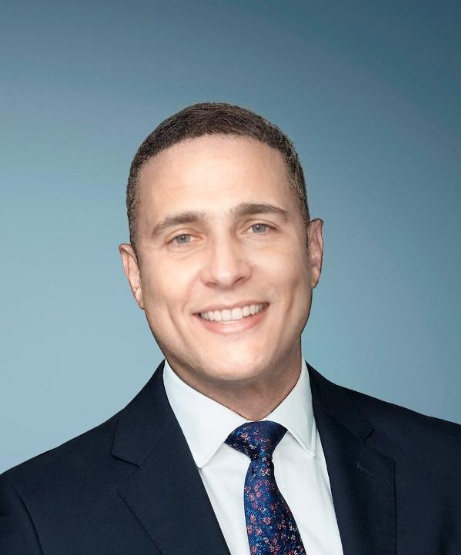
\includegraphics[width=0.11\textwidth]{img/pic/lemon-WM-221.jpg}\hfill
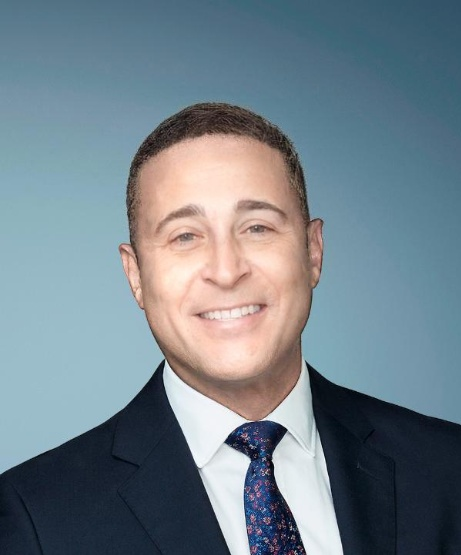
\includegraphics[width=0.11\textwidth]{img/pic/lemon-WM-248.jpg}\hfill
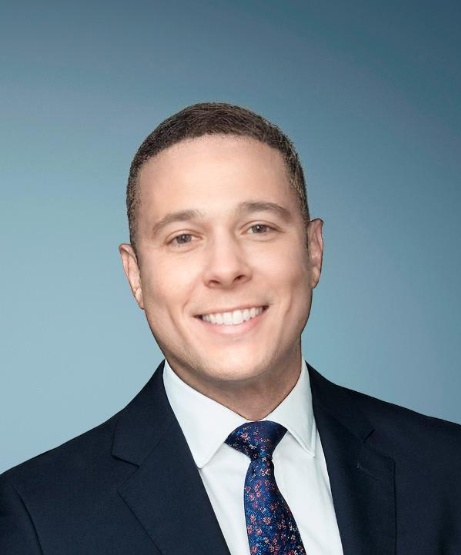
\includegraphics[width=0.11\textwidth]{img/pic/lemon-WM-214.jpg}\hfill
\\ 
\centering
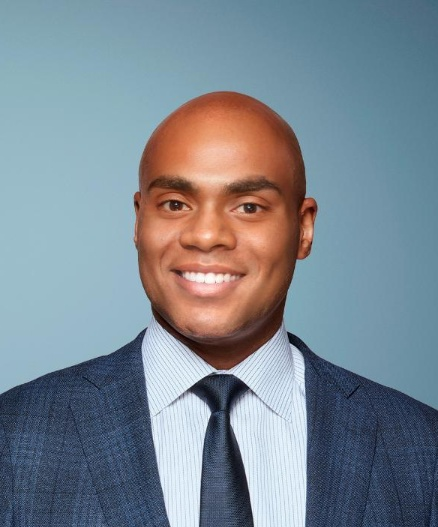
\includegraphics[width=0.11\textwidth]{img/pic/brunhuber-BM-011.jpg}\hfill
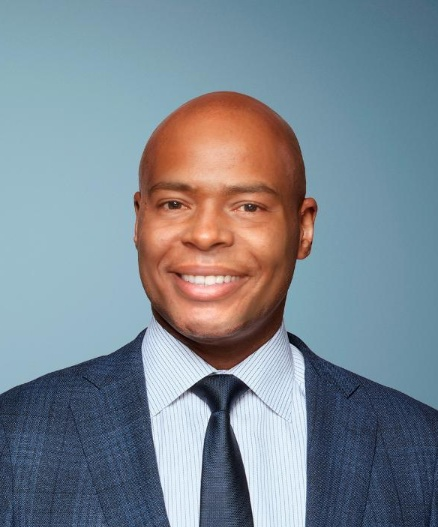
\includegraphics[width=0.11\textwidth]{img/pic/brunhuber-BM-033.jpg}\hfill
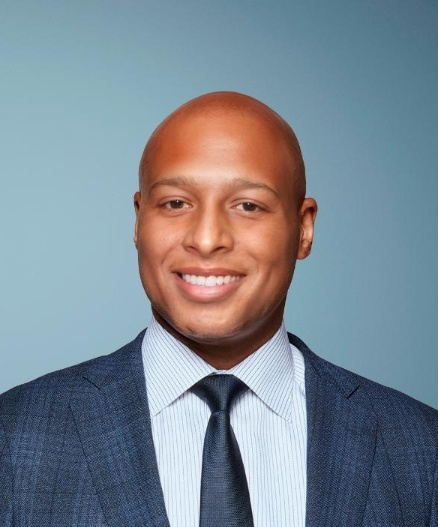
\includegraphics[width=0.11\textwidth]{img/pic/brunhuber-BM-214.jpg}\hfill
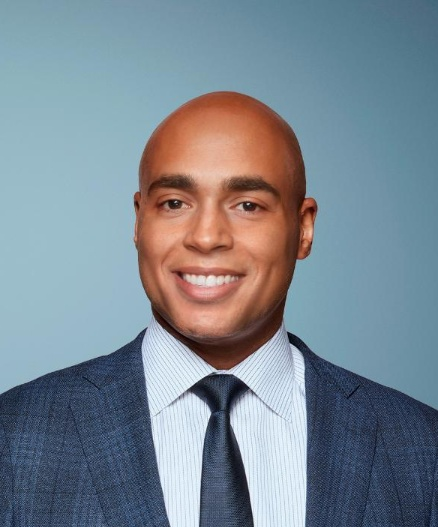
\includegraphics[width=0.11\textwidth]{img/pic/brunhuber-BM-204.jpg}\hfill
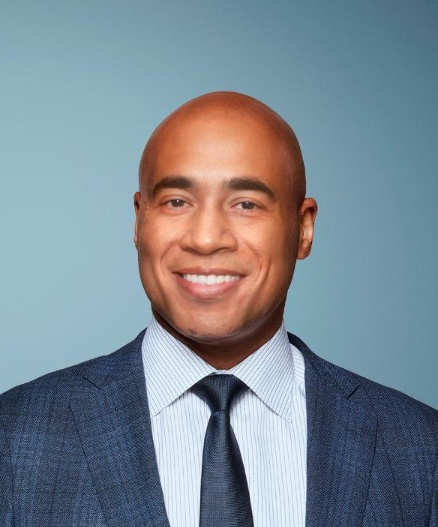
\includegraphics[width=0.11\textwidth]{img/pic/brunhuber-BM-212.jpg}\hfill
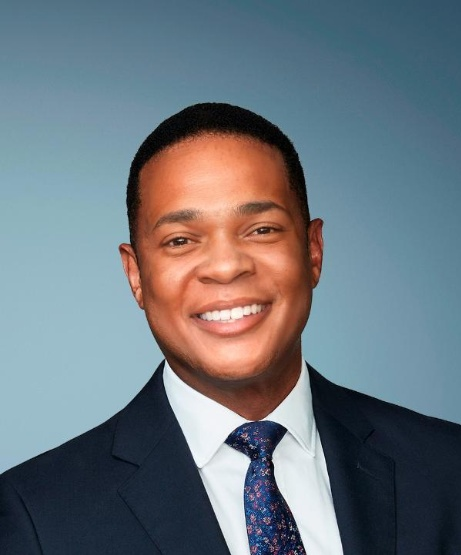
\includegraphics[width=0.11\textwidth]{img/pic/lemon-BM-017.jpg}\hfill
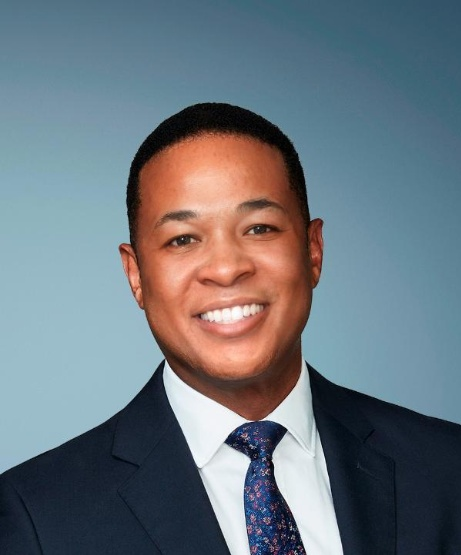
\includegraphics[width=0.11\textwidth]{img/pic/lemon-BM-225.jpg}\hfill
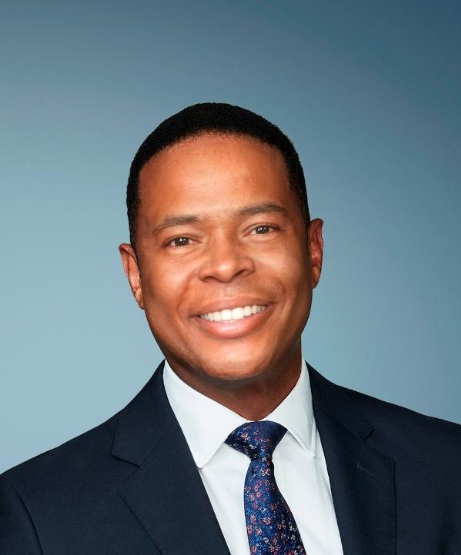
\includegraphics[width=0.11\textwidth]{img/pic/lemon-BM-033.jpg}\hfill
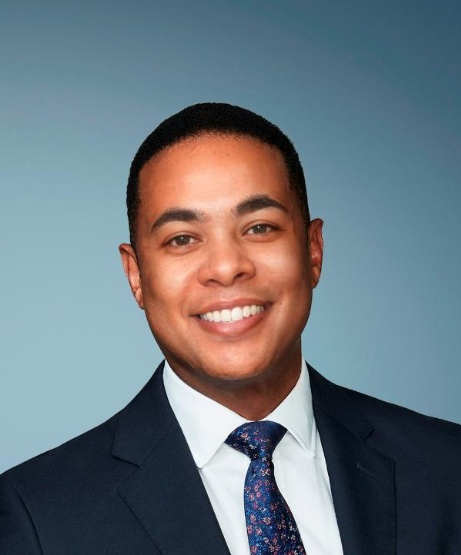
\includegraphics[width=0.11\textwidth]{img/pic/lemon-BM-024.jpg}\hfill
\\
\centering
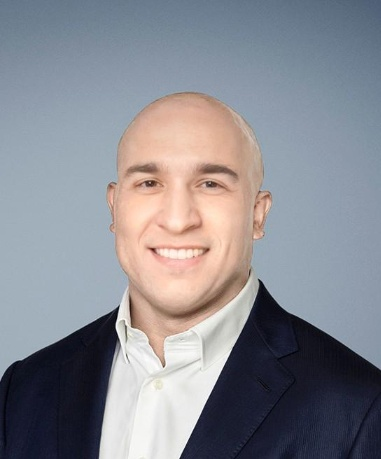
\includegraphics[width=0.11\textwidth]{img/pic/ward-WM-218.jpg}\hfill
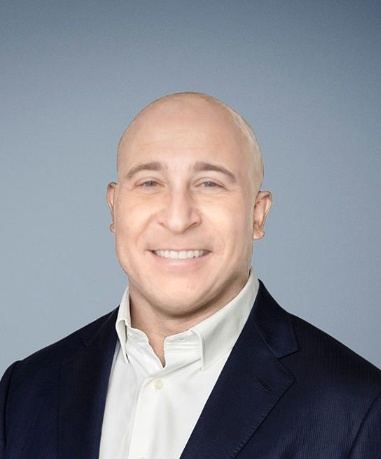
\includegraphics[width=0.11\textwidth]{img/pic/ward-WM-248.jpg}\hfill
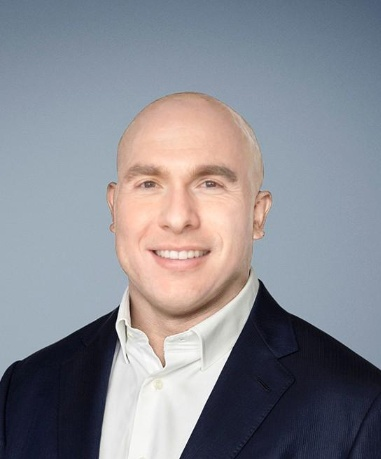
\includegraphics[width=0.11\textwidth]{img/pic/ward-WM-238.jpg}\hfill
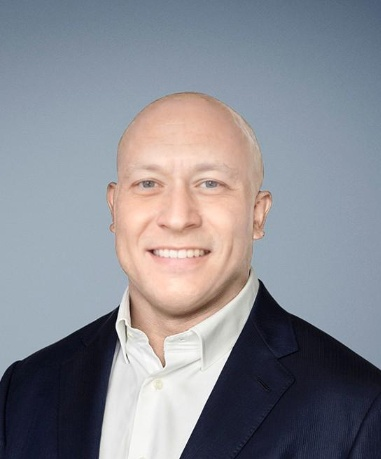
\includegraphics[width=0.11\textwidth]{img/pic/ward-WM-249.jpg}\hfill
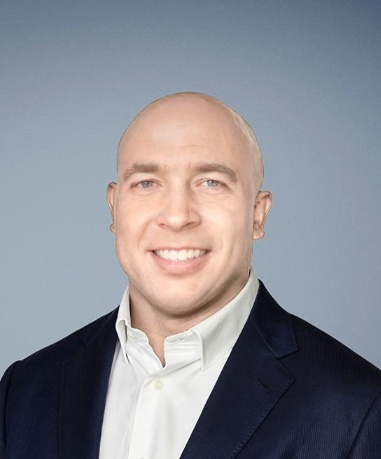
\includegraphics[width=0.11\textwidth]{img/pic/ward-WM-018.jpg}\hfill
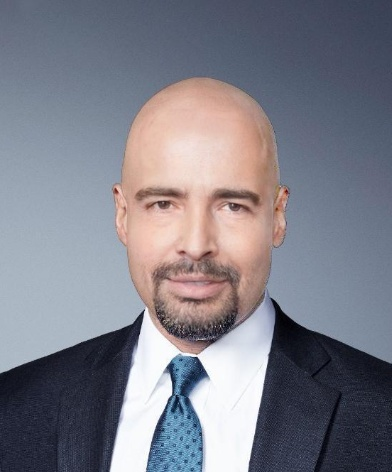
\includegraphics[width=0.11\textwidth]{img/pic/blackwell-WM-211.jpg}\hfill
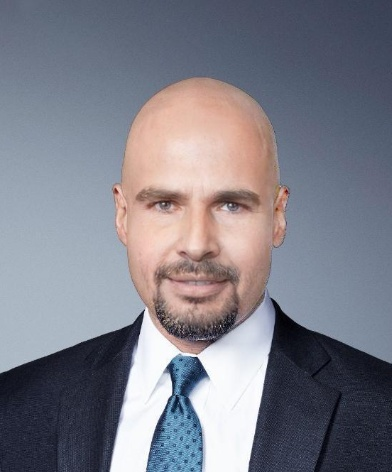
\includegraphics[width=0.11\textwidth]{img/pic/blackwell-WM-241.jpg}\hfill

\includegraphics[width=0.11\textwidth]{img/pic/blackwell-WM-214.jpg}\hfill
\includegraphics[width=0.11\textwidth]{img/pic/blackwell-WM-018.jpg}

\\ 
\centering
\includegraphics[width=0.11\textwidth]{img/pic/ward-BM-227.jpg}\hfill
\includegraphics[width=0.11\textwidth]{img/pic/ward-BM-033.jpg}\hfill
\includegraphics[width=0.11\textwidth]{img/pic/ward-BM-011.jpg}\hfill
\includegraphics[width=0.11\textwidth]{img/pic/ward-BM-245.jpg}\hfill
\includegraphics[width=0.11\textwidth]{img/pic/ward-BM-208.jpg}\hfill
\includegraphics[width=0.11\textwidth]{img/pic/blackwell-BM-208.jpg}\hfill
\includegraphics[width=0.11\textwidth]{img/pic/blackwell-BM-251.jpg}\hfill
\includegraphics[width=0.11\textwidth]{img/pic/blackwell-BM-212.jpg}\hfill
\includegraphics[width=0.11\textwidth]{img/pic/blackwell-BM-017.jpg}

\end{figure}
\end{adjustwidth}
\vspace{-2cm}
\end{frame}
}









\begin{frame}{Neutral Voice}
\label{voice}
\centering
\includegraphics[width=0.8\textwidth]{output/Voice_hist.png}
\vspace{-0.1cm}
	\begin{itemize}
 		\item Respondents distinguish Black and White voice
            \item Respondents cannot distinguish between Experiment and Black and White voice as well
	    \item Respondents cannot distinguish between Experiment and Whitaker's voice used as benchmark 
	\end{itemize}
	
  \hfill \hyperlink{Video_info}{\beamerbutton{Back}}
\end{frame}




\begin{frame}[fragile]{Elicited priors and posteriors}
\label{facts}
\begin{columns}
\column{0.75\textwidth}
    \begin{itemize}
      \item \tikzmark{a}Uninsured U.S. population in 2020: 8.6\%
      \item U.S. population covered by a public program in 2020: 34.8\% 
      \item U.S. population covered by a private program in 2020: 66.5\%   \tikzmark{b}
      \item Percentage of people reporting forgoing medical care due to costs in October 2021: 30\% \tikzmark{f}\tikzmark{g}
      \item Due to fear of COVID-19, part of U.S. population decided to forgo medical care. \tikzmark{c}
      \begin{itemize}
      \item Percentage of U.S. population: 40.9\%
      \item Percentage of White U.S. population: 36.2\%  
      \item Percentage of Hispanic U.S. population: 55.5\%  
      \item Percentage of Black U.S. population: 48.1\% 
      \item Percentage of Asian U.S. population: 37.75\%  \tikzmark{d}
  \end{itemize}
  \end{itemize}
\column{0.25\textwidth}
\begin{tikzpicture}[remember picture,overlay]
\draw[decorate,decoration={brace,raise=12pt}]
  ([yshift=2ex,xshift=5.5cm]{{pic cs:b}|-{pic cs:a}}) --
    node[xshift=1cm,anchor=west]{U.S Census} 
  ([yshift=-0.5ex,xshift=5.5cm]pic cs:b);
\draw[decorate,decoration={brace,raise=12pt}]
  ([yshift=3ex,xshift=1cm]{{pic cs:d}|-{pic cs:c}}) --
    node[xshift=1cm,anchor=west] {CDC report} 
  ([yshift=-0.5ex,xshift=1cm]pic cs:d);
\draw[decorate,decoration={brace,raise=12pt}]
  ([yshift=4ex,xshift=0.5cm]{{pic cs:g}|-{pic cs:f}}) --
    node[xshift=1cm,anchor=west] {Gallup survey} 
  ([yshift=0.5ex,xshift=0.5cm]pic cs:g);

\end{tikzpicture}
\end{columns}
  \hfill \hyperlink{Video_info}{\beamerbutton{Back}}

\end{frame}


\begin{frame}{Measures to avoid cheating}
\label{cheating}
	\begin{itemize}
	    \item Information difficult to retrieve
		\item Self-reported measure
		\item Subjects have limited control over embedded video and have a time limit to watch it (4minutes and 25 seconds)
		\item Priors and posteriors about signal have a time limit after which they do not get paid (45, 20 sec respectively)
	\end{itemize}
 \hfill \hyperlink{Video_info}{\beamerbutton{Back}}

\end{frame}

\begin{frame}{Picture Manipulation - Procedure}
\only<1>{
\begin{figure}[h!]
\begin{minipage}{0.45\columnwidth}
\centering
\captionsetup[subfloat]{labelformat=empty}
\subfloat[Original Victor Blackwell]{\includegraphics[height=4cm]{img/pic/Blackwell originaljpg.jpg}}
\end{minipage}
\begin{minipage}{0.51\columnwidth}
\subfloat{
\includegraphics[height=3.5cm]{img/pic/blackwell-BM-017.jpg}
\includegraphics[height=3.5cm]{img/pic/blackwell-WM-018.jpg}}
\captionsetup[subfloat]{labelformat=empty}
\subfloat[Example of Resulting Pairs]{
\includegraphics[height=3.5cm]{img/pic/blackwell-BM-208.jpg}
\includegraphics[height=3.5cm]{img/pic/blackwell-WM-211.jpg}}
\end{minipage}
\end{figure}
}
\only<2>{
\label{pic_Manipulation}
	\begin{figure}[]
		\centering
		\tikzstyle{box} = [align=left, node distance = 2em]		
		\begin{tikzpicture}[mymat/.style={matrix of nodes,
			draw=none,nodes={draw,rounded corners, align=left, text width=4.5,
				anchor=south},
			row sep=2em,column sep=2em,
			matrix horizontal arrows={-latex}}]
		%\node[box] (r) at (-1,1) {Rectangle};

			\node[box, text width=3.5em] (n1) at (-10,4)  {Picture of body};
			\node[box, text width=3.5em] (n2) at (-10,0.5)  {Picture of face};
			\node[box, right= of n1] (n3) {Photo editing to \\vary gender and race};
			\node[box, right = of n2] (n4) {Chicago \\ Face \\ Database};
		\node[box, right = of n4] (n5) {Calculate pairs on \\ appropriate subsamples \\  using similarity  measures};
			\coordinate (Q) at ([xshift=1cm,yshift=2cm]n5);
	
		\node[box, right = of Q] (N) {Resulting \\ Pairs};
		\node[box, above = of N] (N1) {Survey \\ Validation};	
	
			\draw [->] (n1) -- (n3);
			\draw [->] (n2) -- (n4);
			\draw [->] (Q) -- node[xshift=-0.4cm,above]{swap}(N);
			\draw[in=180,out=0] (n3) to (Q);
			\draw[in=180,out=0] (n5) to (Q);
			\draw[->,bend right] ([xshift=0.1cm]N.north) to ([xshift=0.1cm]N1.south);
			\draw[->,bend right] ([xshift=-0.1cm]N1.south) to ([xshift=-0.1cm]N.north);
		\end{tikzpicture}
	\end{figure}
 }
 \hfill \hyperlink{pic examples}{\beamerbutton{Back}}
\end{frame}

\begin{frame}{Data}
\begin{adjustbox}{width=\textwidth, totalheight=\textheight-\baselineskip,keepaspectratio}

    \begin{tabular}[t]{lllrrr}
\toprule
  & Main Analysis &    & Black
Presenter & White
Presenter & All\\
\midrule
Black Respondents & No & N & 43 & 40 & 83\\
 &  & Percent & \num{2.09} & \num{1.94} & \num{4.03}\\
 & Yes & N & 475 & 477 & 952\\
 &  & Percent & \num{23.04} & \num{23.13} & \num{46.17}\\
 & All & N & 518 & 517 & 1035\\
White Respondents & No & N & 24 & 41 & 65\\
 &  & Percent & \num{1.16} & \num{1.99} & \num{3.15}\\
 & Yes & N & 489 & 473 & 962\\
 &  & Percent & \num{23.71} & \num{22.94} & \num{46.65}\\
 & All & N & 513 & 514 & 1027\\
\bottomrule
\end{tabular}
\end{adjustbox}
\end{frame}


\begin{frame}{Balance Table}
\label{balance}
\resizebox{\textwidth}{!}{
\begin{threeparttable}
\begin{tabular}[t]{lrrrrrr}
\toprule
\multicolumn{1}{c}{ } & \multicolumn{2}{c}{\makecell[c]{Black\\Presenter} (N=1031)} & \multicolumn{2}{c}{\makecell[c]{White\\Presenter} (N=1031)} & \multicolumn{2}{c}{ } \\
\cmidrule(l{3pt}r{3pt}){2-3} \cmidrule(l{3pt}r{3pt}){4-5}
  & Mean & SD & Mean & SD & Mean Diff. & p-value\\
\midrule
Age & 40.086 & 12.524 & 39.790 & 12.554 & -0.295 & 0.599\\
Female & 0.468 & 0.499 & 0.484 & 0.500 & 0.016 & 0.454\\
Immigrant & 0.133 & 0.340 & 0.135 & 0.342 & 0.002 & 0.892\\
At least bachelor degree & 0.526 & 0.500 & 0.540 & 0.499 & 0.015 & 0.506\\
Employed & 0.636 & 0.481 & 0.627 & 0.484 & -0.010 & 0.650\\
Income in $\$\left[0,50\right]$ (th) & 0.387 & 0.487 & 0.363 & 0.481 & -0.024 & 0.256\\
Income in $\$\left[50,100\right]$ (th) & 0.300 & 0.458 & 0.345 & 0.476 & 0.046** & 0.027\\
Democrat & 0.533 & 0.499 & 0.514 & 0.500 & -0.019 & 0.377\\
Republican & 0.134 & 0.341 & 0.138 & 0.345 & 0.004 & 0.800\\
Voted in 2020 & 0.722 & 0.448 & 0.721 & 0.449 & -0.001 & 0.959\\
Hispanic & 0.075 & 0.263 & 0.094 & 0.292 & 0.019 & 0.113\\
Self-reported cheating & 0.065 & 0.247 & 0.079 & 0.269 & 0.014 & 0.232\\
\bottomrule
\end{tabular}
\begin{tablenotes}
\item \textit{Note: } 
\item * p $<$ 0.1, ** p $<$ 0.05, *** p $<$ 0.01. Test of equality of means calculated with standard errors corrected for block sampling.
\end{tablenotes}
\end{threeparttable}
}
\hfill \hyperlink{data}{\beamerbutton{Back}}

\end{frame}

\begin{frame}{Misperceptions - regression}
\label{mainI_reg}
\begin{adjustbox}{width=\textwidth, totalheight=\textheight-\baselineskip,keepaspectratio}

\begin{threeparttable}
\begin{tabular}[t]{lcccccc}
\toprule
\multicolumn{1}{c}{ } & \multicolumn{2}{c}{Presenter/Audience} & \multicolumn{2}{c}{Audience/Info} & \multicolumn{2}{c}{Presenter/Info} \\
\cmidrule(l{3pt}r{3pt}){2-3} \cmidrule(l{3pt}r{3pt}){4-5} \cmidrule(l{3pt}r{3pt}){6-7}
  & (1) & (2) & (3) & (4) & (5) & (6)\\
\midrule
Congruence & \num{-0.003} & \num{0.021} & \num{-1.401}*** & \num{-1.401}*** & \num{-1.326}*** & \num{-1.321}***\\
 & (\num{0.334}) & (\num{0.333}) & (\num{0.194}) & (\num{0.194}) & (\num{0.195}) & (\num{0.195})\\
Black stratum & \num{4.457}*** & \num{4.626}*** & \num{2.804}*** & \num{2.886}*** & \num{2.802}*** & \num{2.885}***\\
 & (\num{0.334}) & (\num{0.338}) & (\num{0.418}) & (\num{0.425}) & (\num{0.418}) & (\num{0.425})\\
Black video &  &  & \num{0.009} & \num{-0.006} & \num{0.011} & \num{-0.004}\\
 &  &  & (\num{0.417}) & (\num{0.415}) & (\num{0.417}) & (\num{0.415})\\
Constant & \num{10.630}*** & \num{9.994}*** & \num{9.655}*** & \num{11.016}*** & \num{9.635}*** & \num{11.000}***\\
 & (\num{0.281}) & (\num{0.782}) & (\num{0.350}) & (\num{0.936}) & (\num{0.350}) & (\num{0.938})\\
\midrule
N & \num{17026} & \num{17026} & \num{7570} & \num{7570} & \num{7570} & \num{7570}\\
Adj.R$2$ & \num{0.026} & \num{0.030} & \num{0.017} & \num{0.024} & \num{0.017} & \num{0.024}\\
Demographic\\controls & No & Yes & No & Yes & No & Yes\\
\bottomrule
\multicolumn{7}{l}{\rule{0pt}{1em}* p $<$ 0.05, ** p $<$ 0.01, *** p $<$ 0.001}\\
\end{tabular}
\begin{tablenotes}[para]
\item \textit{Note: } 
\item Standard errors in parenthesis are clustered at the individual level. 
            Observations are at the individual-fact level. 
\end{tablenotes}
\end{threeparttable}
               \end{adjustbox}
 \hfill \hyperlink{mainI}{\beamerbutton{Back}}
\end{frame}



\begin{frame}{Learning rates - regression}
\label{mainII_reg}
\begin{adjustbox}{width=\textwidth, totalheight=\textheight-\baselineskip,keepaspectratio}
\begin{threeparttable}
\begin{tabular}[t]{lcccccc}
\toprule
\multicolumn{1}{c}{ } & \multicolumn{2}{c}{Presenter/Audience} & \multicolumn{2}{c}{Audience/Info} & \multicolumn{2}{c}{Presenter/Info} \\
\cmidrule(l{3pt}r{3pt}){2-3} \cmidrule(l{3pt}r{3pt}){4-5} \cmidrule(l{3pt}r{3pt}){6-7}
  & (1) & (2) & (3) & (4) & (5) & (6)\\
\midrule
$s-pr$ & \num{0.765}*** & \num{0.763}*** & \num{0.819}*** & \num{0.724}*** & \num{0.818}*** & \num{0.723}***\\
 & (\num{0.015}) & (\num{0.040}) & (\num{0.019}) & (\num{0.050}) & (\num{0.019}) & (\num{0.050})\\
$s-pr\times$Congruence & \num{-0.008} & \num{-0.007} & \num{0.060}*** & \num{0.057}*** & \num{0.063}*** & \num{0.064}***\\
 & (\num{0.018}) & (\num{0.018}) & (\num{0.015}) & (\num{0.015}) & (\num{0.015}) & (\num{0.015})\\
$s-pr\times$Black stratum & \num{-0.159}*** & \num{-0.161}*** & \num{-0.117}*** & \num{-0.115}*** & \num{-0.114}*** & \num{-0.112}***\\
 & (\num{0.018}) & (\num{0.018}) & (\num{0.023}) & (\num{0.024}) & (\num{0.023}) & (\num{0.024})\\
$s-pr\times$Black video &  &  & \num{0.008} & \num{0.008} & \num{0.004} & \num{0.004}\\
 &  &  & (\num{0.023}) & (\num{0.023}) & (\num{0.023}) & (\num{0.023})\\
\midrule
N & \num{17026} & \num{17026} & \num{7570} & \num{7570} & \num{7570} & \num{7570}\\
Adj.R$2$ & \num{0.464} & \num{0.465} & \num{0.622} & \num{0.626} & \num{0.622} & \num{0.626}\\
Demographic\\controls & No & Yes & No & Yes & No & Yes\\
H_0: \beta_0 = 1 & \num{0.000} & \num{0.000} & \num{0.000} & \num{0.000} & \num{0.000} & \num{0.000}\\
\bottomrule
\multicolumn{7}{l}{\rule{0pt}{1em}* p $<$ 0.05, ** p $<$ 0.01, *** p $<$ 0.001}\\
\end{tabular}
\begin{tablenotes}[para]
\item \textit{Note: } 
\item Standard errors in parenthesis are clustered at the individual level. 
            Observations are at the individual-fact level. 
             In the row $H_0: beta_0 = 1$, I report the p-values of a Wald test of the null hypothesis that the coefficient on $s - pr$ is equal to 1.
\end{tablenotes}
\end{threeparttable}
               \end{adjustbox}
 \hfill \hyperlink{mainII}{\beamerbutton{Back}}
\end{frame}


\begin{frame}{Regression Equations}
    \begin{equation}
\label{reg:h1}
    y_{i,f} = \beta_0 x_{i,f}+  \beta_1 x_{i,f}*Congruence1 + \beta_2 x_{i,f}*sample_i + \varepsilon_{i,f}
  \end{equation}
  
\begin{equation}
\label{reg:h2}
    y_{i,f} = \beta_0 x_{i,f}+  \beta_1 x_{i,f} *Congruence2 + \beta_2 x_{i,f} *sample_i + \beta_2 x_{i,f} *presenter_i + \varepsilon_{i,f}
  \end{equation}
  
 \begin{equation}
\label{reg:h3}
    y_{i,f} = \beta_0 x_{i,f}+  \beta_1 x_{i,f}*Congruence3+ \beta_2 x_{i,f} *sample_i + \beta_2 x_{i,f} *presenter_i + \varepsilon_{i,f}
  \end{equation} 

        \begin{description}
\item[$x_{i,f}$] $= \textit{{signal}}_f - \textit{{prior}}_{i,f}$ : difference between signal and prior belief about fact $f$ from individual $i$

\item[$y_{i,f}$] $= \textit{posterior}_{i,f} - \textit{prior}_{i,f}$ : difference between posterior and prior belief about fact $f$ from individual $i$

\item[$sample_{i}$] : indicator for respondent's $i$ race 
\item[$presenter_{i}$] : indicator for respondent's $i$ assigned presenter's race 
      \end{description}
\hfill \hyperlink{eq_learning}
{\beamerbutton{Back}}
\end{frame}

\begin{frame}{Congruence black and white}
\label{congruence_table}
\begin{table}[]
\begin{tabular}{cm{2.1cm}m{2.1cm}m{2.1cm}m{2.1cm}}
                      & \multicolumn{2}{c}{\includegraphics[width=.1\textwidth]{person_white.png}}                          & \multicolumn{2}{c}{\includegraphics[width=.1\textwidth]{person_black.png}}                          \\
                      & \includegraphics[width=.1\textwidth]{presenter_white.png}    
                      &  \includegraphics[width=.1\textwidth]{presenter_black.png}        
                      & \includegraphics[width=.1\textwidth]{presenter_white.png}            &  \includegraphics[width=.1\textwidth]{presenter_black.png}                 \\ \cline{2-5} 
\includegraphics[width=.07\textwidth]{info_white.png} & \multicolumn{1}{|l|}{$C^{i,f}$ , $C^{i,p}$ ,$C^{f,p}$} & \multicolumn{1}{l|}{$C^{i,f}$} & \multicolumn{1}{l|}{$C^{f,p}$} & \multicolumn{1}{l|}{$C^{i,p}$} \\ \cline{2-5} 
\includegraphics[width=.07\textwidth]{info_black.png} & \multicolumn{1}{|l|}{$C^{i,p}$} & \multicolumn{1}{l|}{$C^{f,p}$} & \multicolumn{1}{l|}{$C^{i,f}$} & \multicolumn{1}{l|}{$C^{i,f}$ , $C^{i,p}$ ,$C^{f,p}$} \\ \cline{2-5} 
\includegraphics[width=.07\textwidth]{info_green.png} & \multicolumn{1}{|l|}{$C^{i,p}$} & \multicolumn{1}{l|}{} & \multicolumn{1}{l|}{} & \multicolumn{1}{l|}{$C^{i,p}$} \\ \cline{2-5} 
\includegraphics[width=.07\textwidth]{info_blu.png} & \multicolumn{1}{|l|}{$C^{i,p}$} & \multicolumn{1}{l|}{} & \multicolumn{1}{l|}{} & \multicolumn{1}{l|}{$C^{i,p}$} \\ \cline{2-5} 
\end{tabular}
\end{table}
\end{frame}

\begin{frame}[allowframebreaks]{References}

  \bibliography{}
  \bibliographystyle{abbrv}

\end{frame}

\end{document}


%
%
%
%
%
%
%
%
%
%
%
%
%
%%
%
%
%
%
%
%%
%
%
%
%
%
%%
%
%
%
%
%
%%
%
%
%
%
%
%%
%
%
%
%
%
%


\begin{frame}{Priors - general information}
	\begin{itemize}
		\item What do you think was the percentage of Americans who were without health insurance in 2020?
		\item What do you think was the percentage of Americans in 2020 who got their health insurance coverage through a \textbf{federal or state programs} such as Medicaid or Medicare?
		\item What do you think was the percentage of Americans in 2020 who got their health insurance coverage through a \textbf{private program} such as employment-based coverage, direct-purchase or military?
		\item Due to rising medical costs, many people in the United States decided to forgo medical care at some point in 2021.\\
        What do you think is the percentage of people that in October 2021 reported doing so?
	\end{itemize}
\end{frame}


\begin{frame}{Priors - information for racial sub-groupings}
	\begin{itemize}
		\item What do you think was the percentage of Americans who were without health insurance in 2020?
		\item What do you think was the percentage of Americans in 2020 who got their health insurance coverage through a \textbf{federal or state programs} such as Medicaid or Medicare?
		\item What do you think was the percentage of Americans in 2020 who got their health insurance coverage through a \textbf{private program} such as employment-based coverage, direct-purchase or military?
		\item Due to rising medical costs, many people in the United States decided to forgo medical care at some point in 2021.\\
        What do you think is the percentage of people that in October 2021 reported doing so?
	\end{itemize}
\end{frame}


\begin{frame}{Conceptual Framework}
Gabaix (2019)'s model

\begin{equation*}
    x_i^s := m_ix_i+(1-m_i)x_i^d
\end{equation*}
\begin{description}
  \item[$x_i^s$] Subjectively perceived variable $x_i$
  \item[$x_i^d$] Default value for variable $x_i$ (e.g. the prior)
  \item[$x_i$] True value for variable $x_i$
   \alert{\item[$m_i$] Attention} to variable $x_i$, with $m_i \in \left[0,1\right]$
\end{description}
\only<2>{
In DellaVigna (2009), 
\begin{equation*}
    m := f(\gamma,N)
\end{equation*}
\begin{description}
  \item[$\gamma$] Salience of the signal
  \item[$N$] Number of competing stimuli
\end{description}}
\end{frame}

\begin{frame}{Congruence black and white}
\begin{table}[]
  \begin{tabular}{|c|c|c|c|}
      \hline
\begin{tikzpicture}[scale=0.2]
\node[inner sep=0pt] (info) at (0,-4)
    {\includegraphics[width=.050\textwidth]{info_black.png}};
\node[inner sep=0pt] (person) at (3.5,0)
    {\includegraphics[width=.050\textwidth]{person_black.png}};
\node[inner sep=0pt] (presenter) at (7,-4)
    {\includegraphics[width=.050\textwidth]{presenter_black.png}};
\draw[<->,thick] (person.south west) -- (info.north east);
\draw[<->,thick] (info.east) -- (presenter.west);
\draw[<->,thick] (person.south east) -- (presenter.north west);
\end{tikzpicture}  &    
\begin{tikzpicture}[scale=0.2]
\node[inner sep=0pt] (info) at (0,-4)
    {\includegraphics[width=.050\textwidth]{info_white.png}};
\node[inner sep=0pt] (person) at (3.5,0)
    {\includegraphics[width=.050\textwidth]{person_black.png}};
\node[inner sep=0pt] (presenter) at (7,-4)
    {\includegraphics[width=.050\textwidth]{presenter_black.png}};
\draw[<->,thick] (person.south west) -- (info.north east);
\draw[<->,thick] (info.east) -- (presenter.west);
\draw[<->,thick] (person.south east) -- (presenter.north west);
\end{tikzpicture} & \begin{tikzpicture}[scale=0.2]
\node[inner sep=0pt] (info) at (0,-4)
    {\includegraphics[width=.050\textwidth]{info_black.png}};
\node[inner sep=0pt] (person) at (3.5,0)
    {\includegraphics[width=.050\textwidth]{person_black.png}};
\node[inner sep=0pt] (presenter) at (7,-4)
    {\includegraphics[width=.050\textwidth]{presenter_white.png}};
\draw[<->,thick] (person.south west) -- (info.north east);
\draw[<->,thick] (info.east) -- (presenter.west);
\draw[<->,thick] (person.south east) -- (presenter.north west);
\end{tikzpicture}  & \begin{tikzpicture}[scale=0.2]
\node[inner sep=0pt] (info) at (0,-4)
    {\includegraphics[width=.050\textwidth]{info_white.png}};
\node[inner sep=0pt] (person) at (3.5,0)
    {\includegraphics[width=.050\textwidth]{person_black.png}};
\node[inner sep=0pt] (presenter) at (7,-4)
    {\includegraphics[width=.050\textwidth]{presenter_white.png}};
\draw[<->,thick] (person.south west) -- (info.north east);
\draw[<->,thick] (info.east) -- (presenter.west);
\draw[<->,thick] (person.south east) -- (presenter.north west);
\end{tikzpicture}  \\ \hline

\begin{tikzpicture}[scale=0.2]
\node[inner sep=0pt] (info) at (0,-4)
    {\includegraphics[width=.050\textwidth]{info_black.png}};
\node[inner sep=0pt] (person) at (3.5,0)
    {\includegraphics[width=.050\textwidth]{person_white.png}};
\node[inner sep=0pt] (presenter) at (7,-4)
    {\includegraphics[width=.050\textwidth]{presenter_black.png}};
\draw[<->,thick] (person.south west) -- (info.north east);
\draw[<->,thick] (info.east) -- (presenter.west);
\draw[<->,thick] (person.south east) -- (presenter.north west);
\end{tikzpicture}   &   \begin{tikzpicture}[scale=0.2]
\node[inner sep=0pt] (info) at (0,-4)
    {\includegraphics[width=.050\textwidth]{info_white.png}};
\node[inner sep=0pt] (person) at (3.5,0)
    {\includegraphics[width=.050\textwidth]{person_white.png}};
\node[inner sep=0pt] (presenter) at (7,-4)
    {\includegraphics[width=.050\textwidth]{presenter_black.png}};
\draw[<->,thick] (person.south west) -- (info.north east);
\draw[<->,thick] (info.east) -- (presenter.west);
\draw[<->,thick] (person.south east) -- (presenter.north west);
\end{tikzpicture}  & \begin{tikzpicture}[scale=0.2]
\node[inner sep=0pt] (info) at (0,-4)
    {\includegraphics[width=.050\textwidth]{info_black.png}};
\node[inner sep=0pt] (person) at (3.5,0)
    {\includegraphics[width=.050\textwidth]{person_white.png}};
\node[inner sep=0pt] (presenter) at (7,-4)
    {\includegraphics[width=.050\textwidth]{presenter_white.png}};
\draw[<->,thick] (person.south west) -- (info.north east);
\draw[<->,thick] (info.east) -- (presenter.west);
\draw[<->,thick] (person.south east) -- (presenter.north west);
\end{tikzpicture}  & \begin{tikzpicture}[scale=0.2]
\node[inner sep=0pt] (info) at (0,-4)
    {\includegraphics[width=.050\textwidth]{info_white.png}};
\node[inner sep=0pt] (person) at (3.5,0)
    {\includegraphics[width=.050\textwidth]{person_white.png}};
\node[inner sep=0pt] (presenter) at (7,-4)
    {\includegraphics[width=.050\textwidth]{presenter_white.png}};
\draw[<->,thick] (person.south west) -- (info.north east);
\draw[<->,thick] (info.east) -- (presenter.west);
\draw[<->,thick] (person.south east) -- (presenter.north west);
\end{tikzpicture}    \\ \hline
  \end{tabular}
\end{table}
\end{frame}

\begin{frame}{Congruence}

\label{congruence}
\begin{tikzpicture}
\node[inner sep=0pt] (info) at (0,-4)
    {\includegraphics[width=.25\textwidth]{info_black.png}};
\node[inner sep=0pt] (person) at (3.5,0)
    {\includegraphics[width=.25\textwidth]{person_black.png}};
\node[inner sep=0pt] (presenter) at (7,-4)
    {\includegraphics[width=.25\textwidth]{presenter_black.png}};
\draw[<->,thick] (person.south west) -- (info.north east)
    node[midway,fill=white] {$C^{I,F}$};
\draw[<->,thick] (info.east) -- (presenter.west)
    node[midway,fill=white] {$C^{F,P}$};
\draw[<->,thick] (person.south east) -- (presenter.north west)
    node[midway,fill=white] {$C^{I,P}$};
\end{tikzpicture}
\hfill \hyperlink{m}{\beamerbutton{Back}}
\end{frame}
